\documentclass[compress]{beamer}
\usepackage{ifthen,verbatim}

\newcommand{\isnote}{}
\xdefinecolor{lightyellow}{rgb}{1.,1.,0.25}
\xdefinecolor{darkblue}{rgb}{0.1,0.1,0.7}

%% Uncomment this to get annotations
%% \def\notes{\addtocounter{page}{-1}
%%            \renewcommand{\isnote}{*}
%% 	   \beamertemplateshadingbackground{lightyellow}{white}
%%            \begin{frame}
%%            \frametitle{Notes for the previous page (page \insertpagenumber)}
%%            \itemize}
%% \def\endnotes{\enditemize
%% 	      \end{frame}
%%               \beamertemplateshadingbackground{white}{white}
%%               \renewcommand{\isnote}{}}

%% Uncomment this to not get annotations
\def\notes{\comment}
\def\endnotes{\endcomment}

\setbeamertemplate{navigation symbols}{}
\setbeamertemplate{headline}{\mbox{ } \hfill
\begin{minipage}{5.5 cm}
\vspace{-0.75 cm} \small
\end{minipage} \hfill
\begin{minipage}{4.5 cm}
\vspace{-0.75 cm} \small
\begin{flushright}
\ifthenelse{\equal{\insertpagenumber}{0}}{}{\hspace{0.2 cm} \insertpagenumber\isnote/\pageref{numpages}}
\end{flushright}
\end{minipage}\mbox{\hspace{0.2 cm}}\includegraphics[height=1 cm]{../cmslogo} \hspace{0.1 cm} \includegraphics[height=1 cm]{../tamulogo} \hspace{0.01 cm} \vspace{-1.05 cm}}

\newcommand{\s}[1]{{\mbox{\scriptsize #1}}}

\begin{document}
%% \begin{frame}
%% \vfill
%% \begin{center}
%% \textcolor{darkblue}{\Large TITLE}

%% \vfill
%% \begin{columns}
%% \column{0.3\linewidth}
%% \begin{center}
%% \large
%% Aysen Tatarinov

%% Vadim Khotilovich

%% \textcolor{darkblue}{\it Jim Pivarski}

%% Alexei Safonov
%% \end{center}
%% \end{columns}

%% \begin{columns}
%% \column{0.3\linewidth}
%% \begin{center}
%% \scriptsize
%% {\it Texas A\&M University}
%% \end{center}
%% \end{columns}

%% \vfill
%% 28 February, 2011

%% \end{center}
%% \end{frame}

%% \begin{notes}
%% \item This is the annotated version of my talk.
%% \item If you want the version that I am presenting, download the one
%% labeled ``slides'' on Indico (or just ignore these yellow pages).
%% \item The annotated version is provided for extra detail and a written
%% record of comments that I intend to make orally.
%% \item Yellow notes refer to the content on the {\it previous} page.
%% \item All other slides are identical for the two versions.
%% \end{notes}

\small

%% \begin{frame}
%% \frametitle{Outline}
%% \begin{itemize}\setlength{\itemsep}{0.75 cm}
%% \item 
%% \end{itemize}
%% %% \hspace{-0.83 cm} \textcolor{darkblue}{\Large Outline2}
%% \end{frame}

\begin{frame}
\vfill

\textcolor{darkblue}{\large Question: is the signal efficiency affected by interference between muons in the tracker, possibly in a way that is not well modeled by Monte Carlo?}

\vfill
\textcolor{darkblue}{\large That is, how do we know that our MC-based efficiency is accurate?}

\vfill
\end{frame}

%% \begin{frame}
%% \frametitle{List of studies}

%% \renewcommand{\arraystretch}{2}
%% \begin{tabular}{p{0.3\linewidth} p{0.1\linewidth} p{0.5\linewidth}}
%%  & Page & Purpose \\\hline
%% Facts about tracking & \pageref{page:facts_about_tracking} & Qualitative argument that efficiency loss due to nearby tracks in the tracker is negligible \\

%% $\phi(1020)$ resonance & \pageref{page:phi_study} & Data/MC comparisons of $\Delta R \sim 1$ muons in our sample \\

%% Very nearby muons & \pageref{page:very_nearby} & MC study of $\Delta R < 0.05$ muons, search for onset of inefficiency \\
%% \end{tabular}
%% \end{frame}

\begin{frame}
\frametitle{Facts about tracking}
\label{page:facts_about_tracking}

\begin{itemize}
\item Any tracks found in the same iteration can share up to 50\% of hits
\begin{itemize}
\item first two iterations of tracking use pixel triplets and pixel
  seed pairs to find prompt tracks with $p_T > 0.9$~GeV/$c$,
  subsequent iterations are for low-$p_T$ and displaced tracks (not
  our muons)
\end{itemize}

\item To share $\gtrsim$ 50\% of their hits, the two oppositely-charged
  muons must be close enough to merge clusters along most
  of the two tracks

\item For 100~micron-wide pixels at $r=5$~cm and 300~micron-wide
  strips at $r=60$~cm from the beamline, two muons can only get within
  5 pixels {\it and} strips of each other if both muons have $p_T >
  60$~GeV/$c$, within 2 if $p_T > 150$~GeV/$c$, and within 1 if $p_T >
  300$~GeV/$c$
\end{itemize}

\vspace{-0.25 cm}
{\tiny Left: $r\phi$ separation (color) in pixel/strip widths at 5 and 60~cm.  Right: minimum pixel/strip widths at a given $p_T$.}

\mbox{\hspace{-0.5 cm}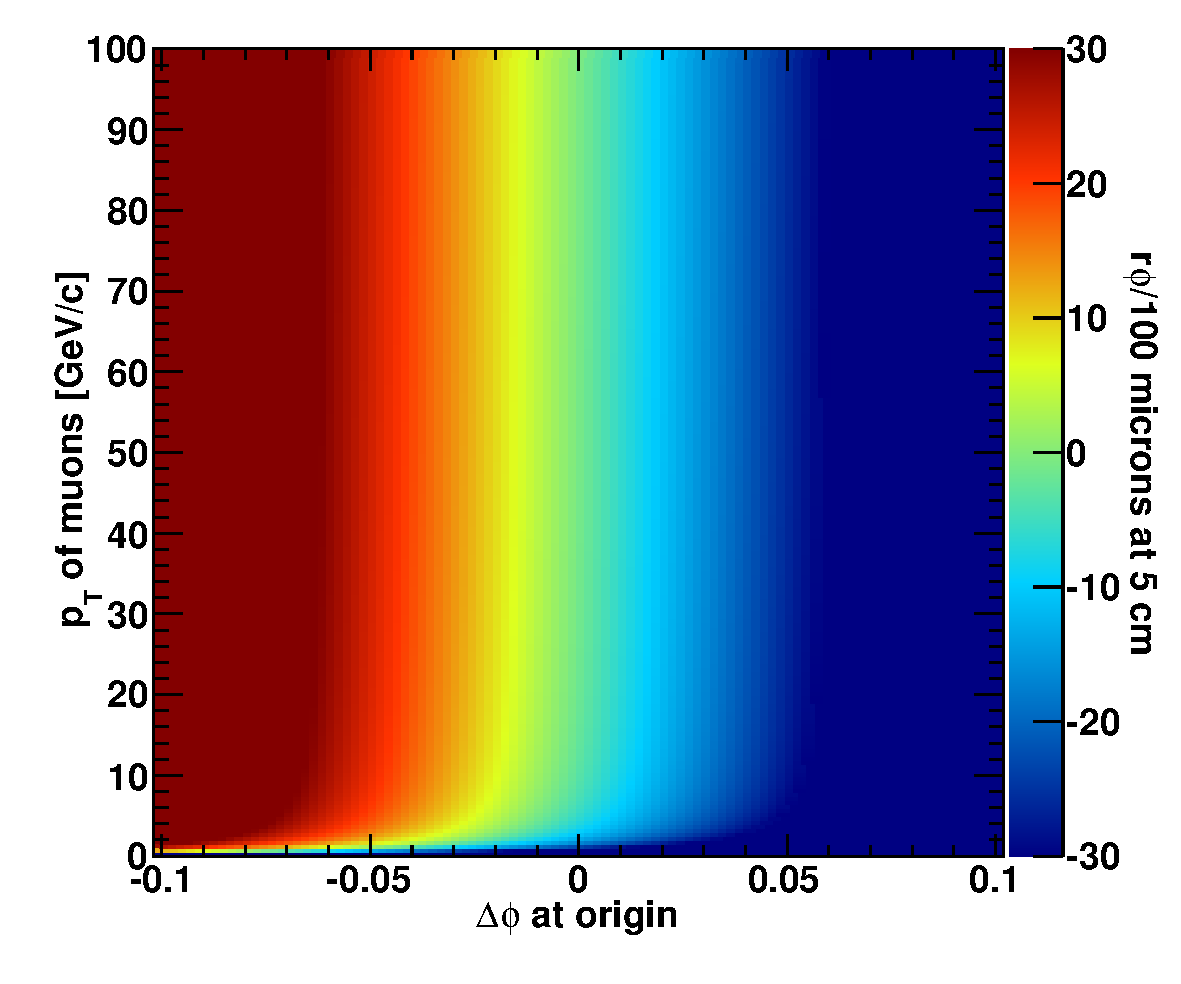
\includegraphics[width=0.38\linewidth]{separation_at_5cm.pdf}
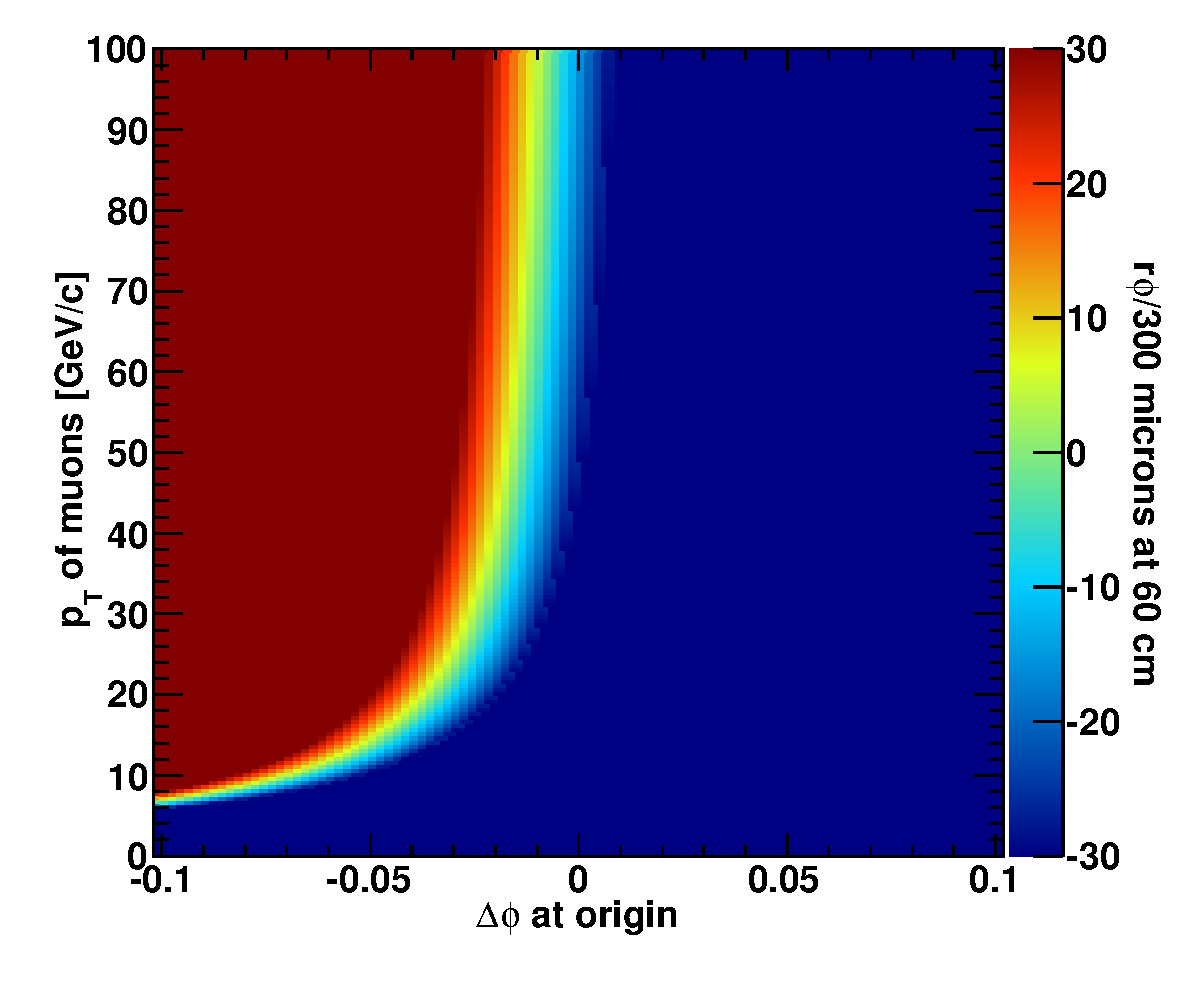
\includegraphics[width=0.38\linewidth]{separation_at_60cm.pdf}
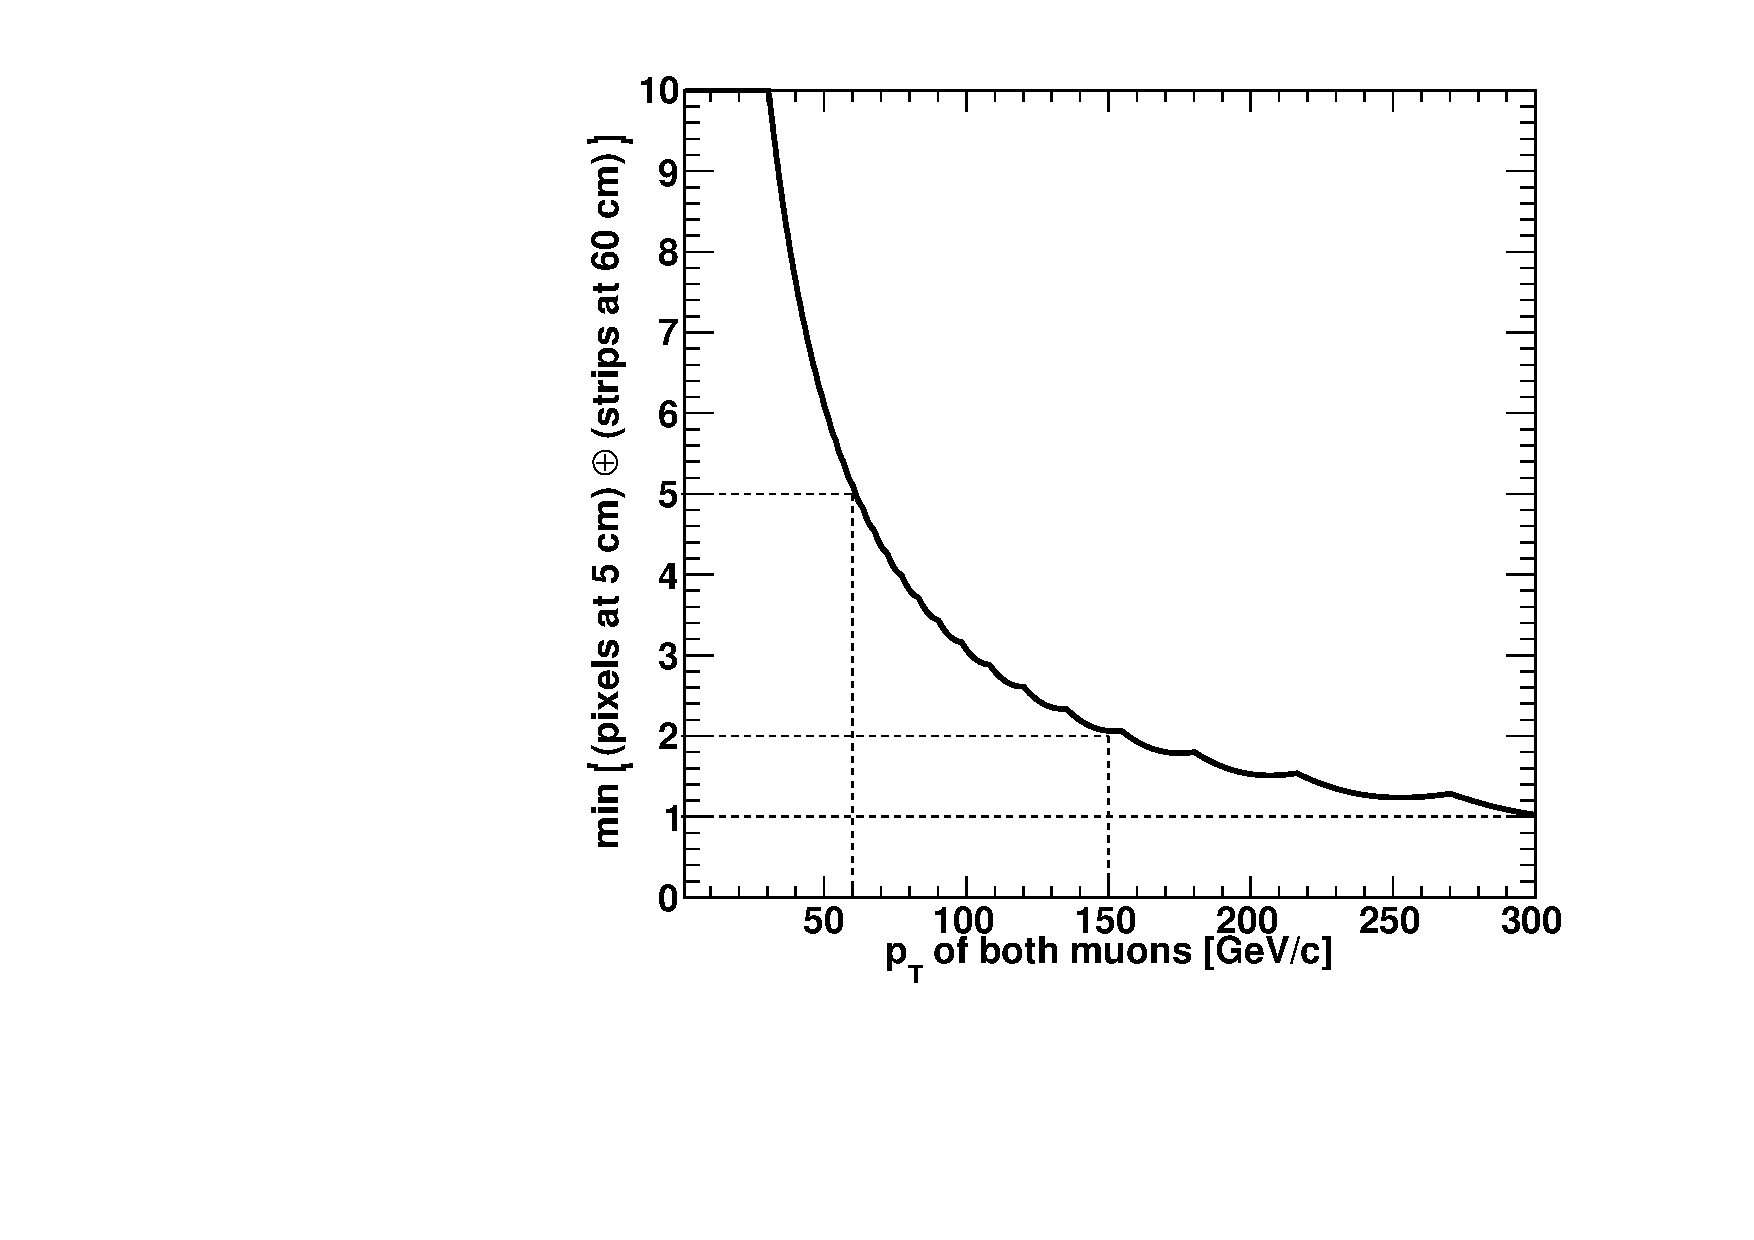
\includegraphics[width=0.38\linewidth]{separation_minimum.pdf}}
\end{frame}

\begin{frame}
\frametitle{Very collinear muons}

Search for the efficiency dip when muons are very close to one another:
\begin{itemize}
\item Pair-gun Monte Carlo through full simulation three times for each pair: once with both $\mu^+$ and $\mu^-$ in the same event, once with only $\mu^+$, and once with only $\mu^-$

\item Define efficiency as: $\displaystyle \frac{\mbox{found tracks individually {\it and} when together}}{\mbox{found tracks individually}}$
\begin{itemize}
\item ``found tracks'' means reconstructed, \#hits $\ge$ 8, $\chi^2/N_\s{dof} < 4$
\item $\sim$equivalent to normal efficiency definition because ``found tracks individually'' is about 99.6\% everywhere \mbox{\scriptsize (always $>$ 99.0\%)}
\end{itemize}
\end{itemize}

\vspace{-0.25 cm}
\begin{columns}
\column{0.45\linewidth}
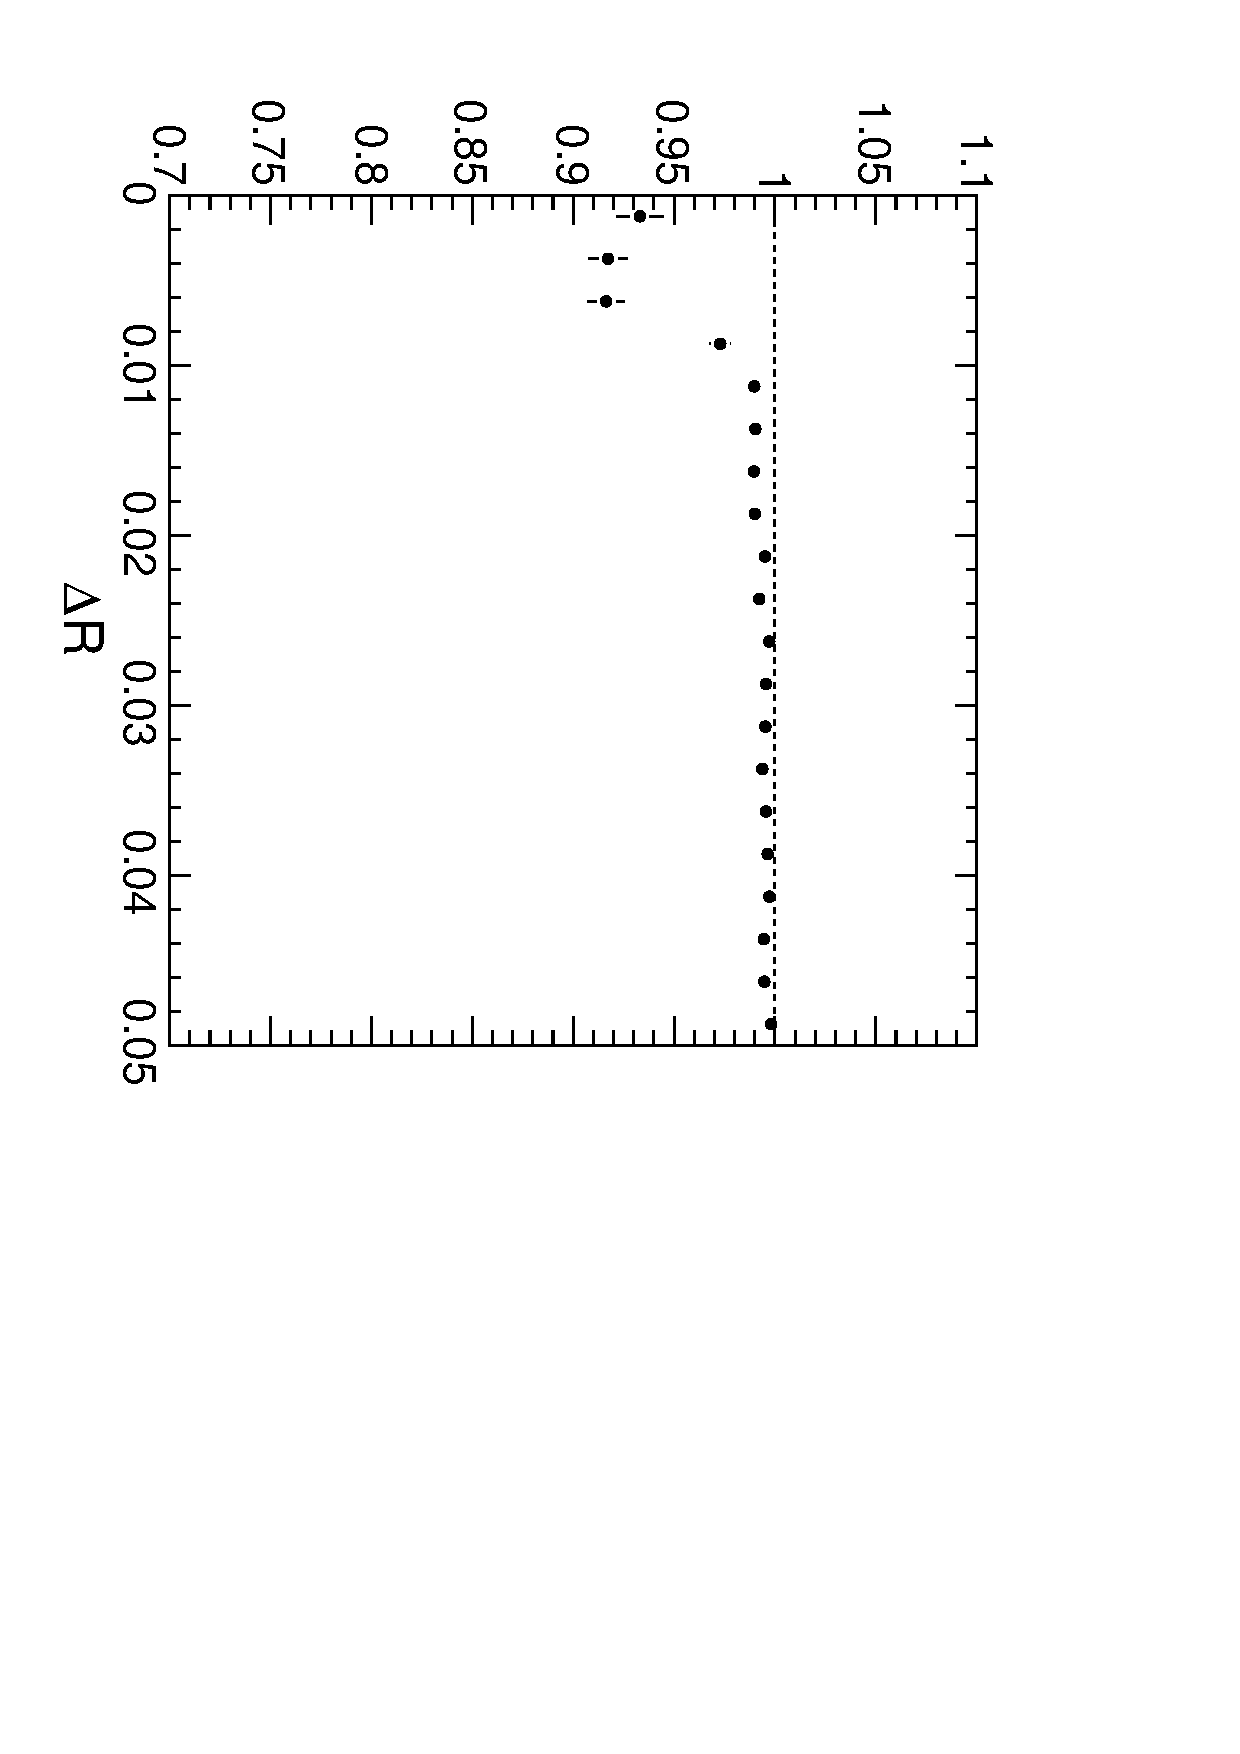
\includegraphics[height=\linewidth, angle=90]{doubleeff_deltar.pdf}
\column{0.45\linewidth}
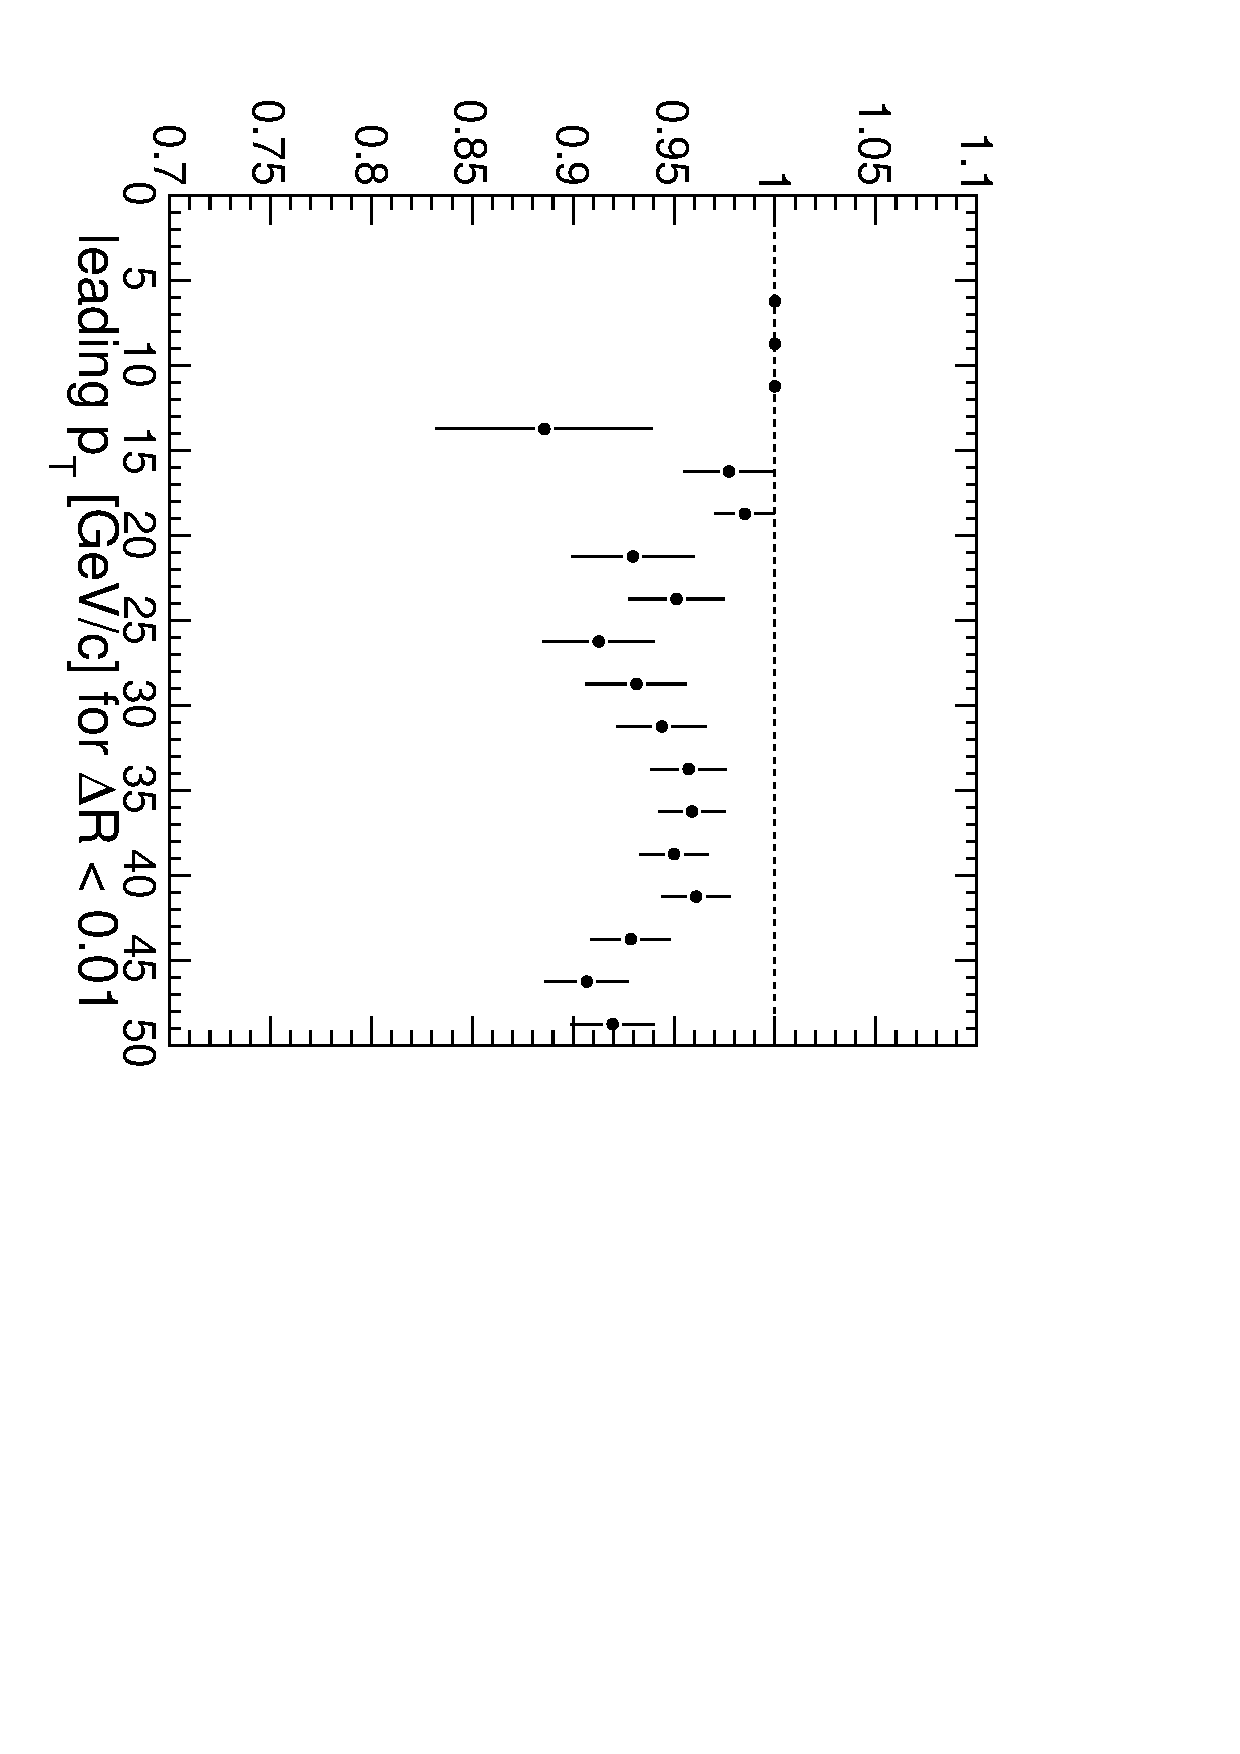
\includegraphics[height=\linewidth, angle=90]{doubleeff_leadpt.pdf}
\column{0.2\linewidth}
\scriptsize 
lose about 5\% in $\Delta R < 0.01$, $p_{T} > 20$~GeV/$c$ that isn't lost when the muons are simulated individually
\end{columns}
\end{frame}

\begin{frame}
\frametitle{Very collinear muons}

Same for muon efficiency:
\begin{itemize}
\item Define efficiency as: $\displaystyle \frac{\mbox{found muons individually {\it and} when together}}{\mbox{found muons individually}}$

\item ``Found muons'' means reconstructed, \#hits $\ge$ 8, $\chi^2/N_\s{dof} < 4$, number of arbitrated segments $\ge$ 2
\end{itemize}

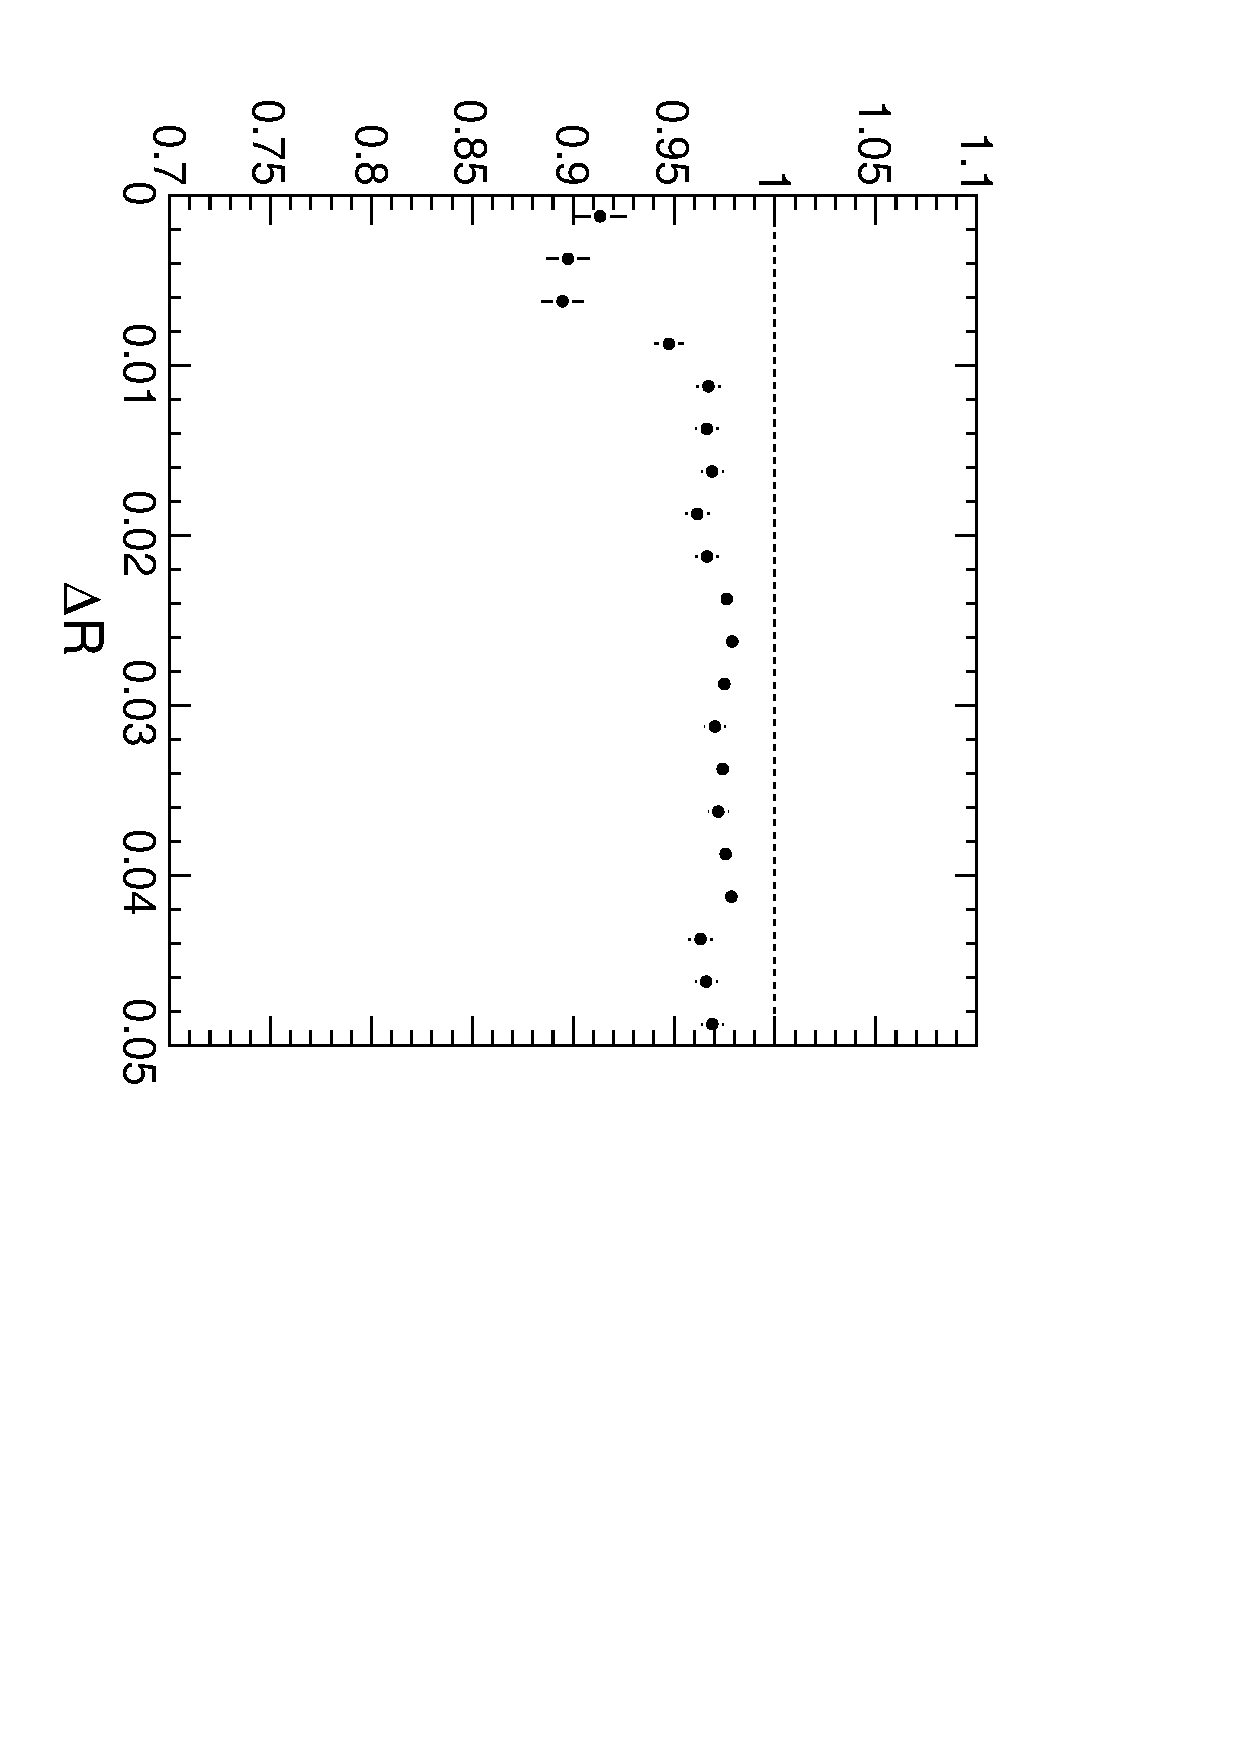
\includegraphics[height=0.4\linewidth, angle=90]{doubleeff_deltar_muon.pdf}
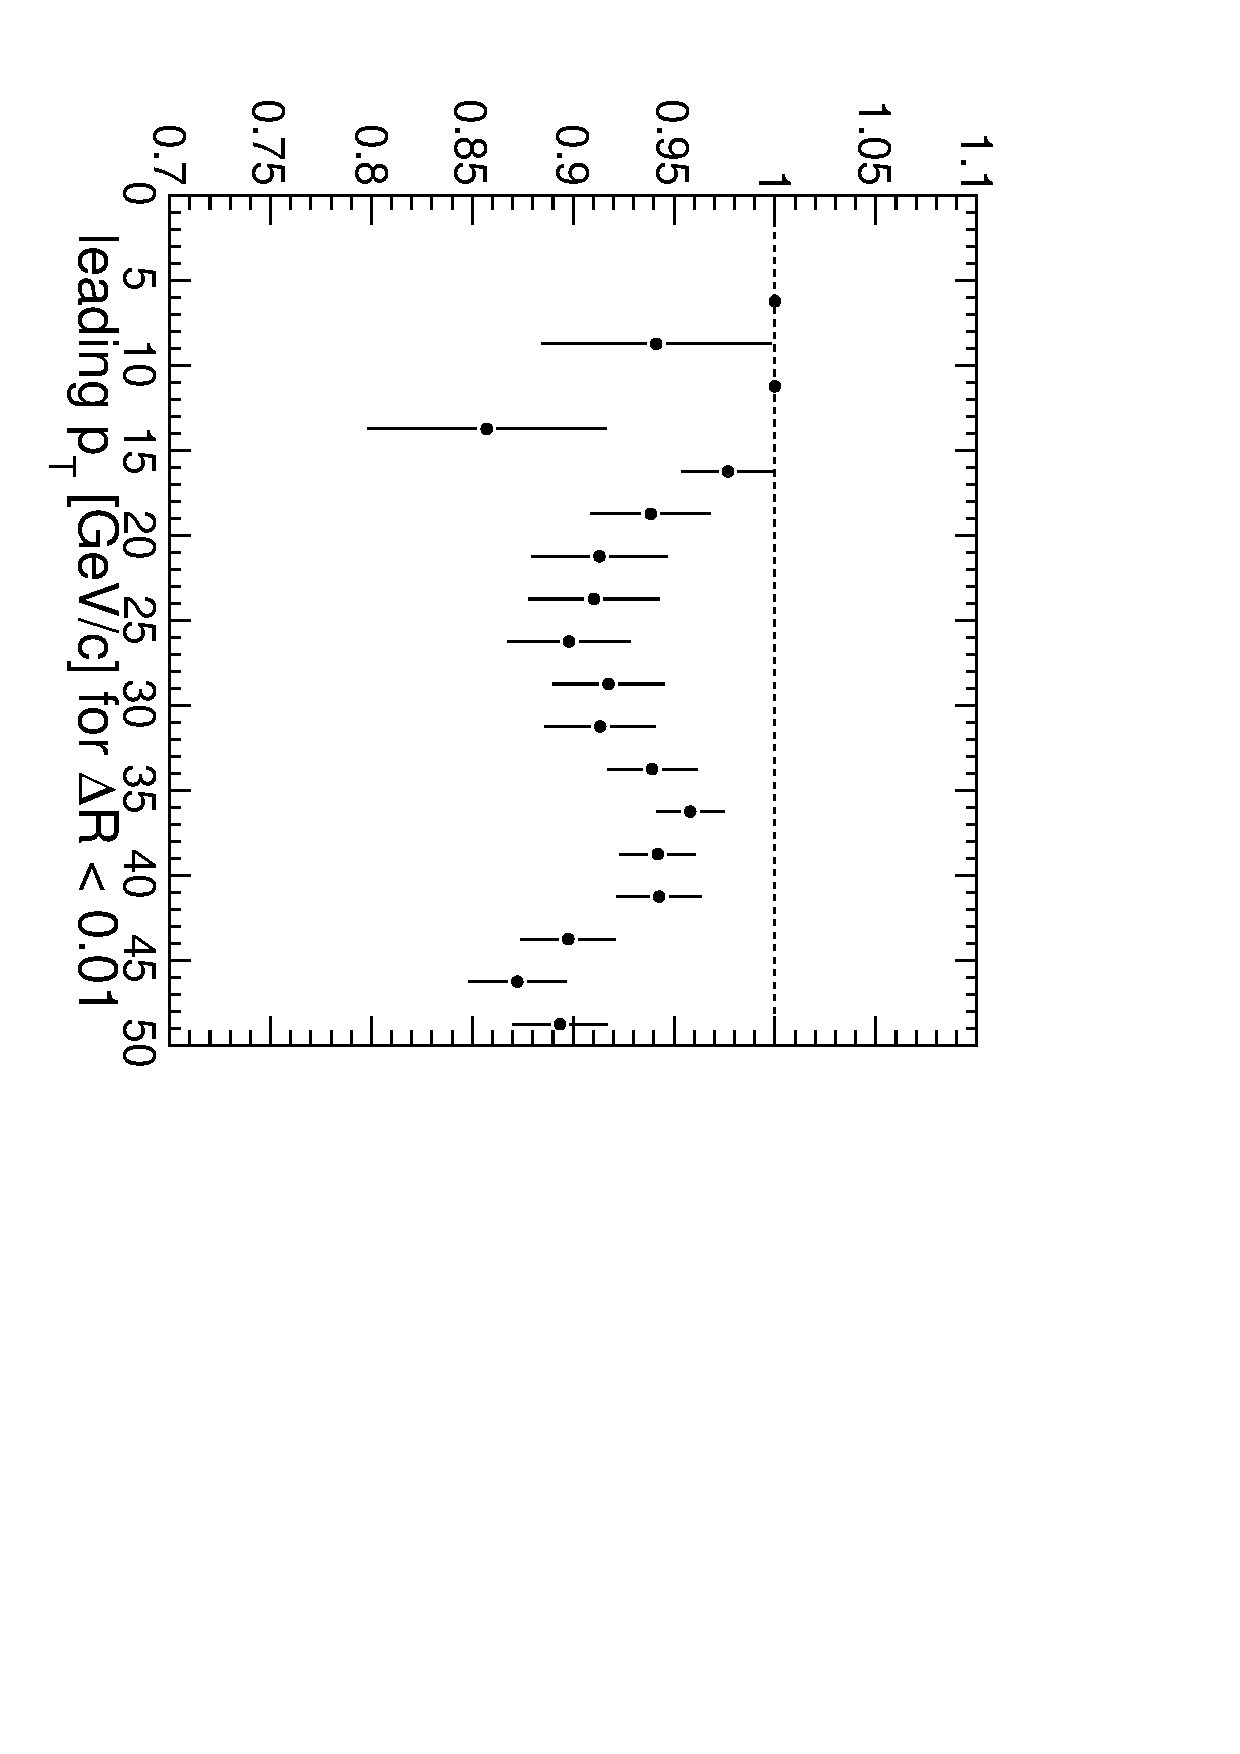
\includegraphics[height=0.4\linewidth, angle=90]{doubleeff_leadpt_muon.pdf}

Conclusion: there is a 5\% tracker-interference effect for $\Delta R < 0.01$ and $p_T > 20$~GeV/$c$, and a muon-interference effect for larger $\Delta R$ values (already documented in analysis note)
\end{frame}

\begin{frame}
\frametitle{Accuracy of the Monte Carlo}

\begin{itemize}
\item Start with data/Monte Carlo comparisons from the Tracker
  DPG early 7 TeV paper (\textcolor{blue}{\url{http://arxiv.org/abs/1007.1988}}):
\begin{itemize}
\item low-level comparisons show we have a good bottom-up simulation
\end{itemize}
\end{itemize}

\begin{center}
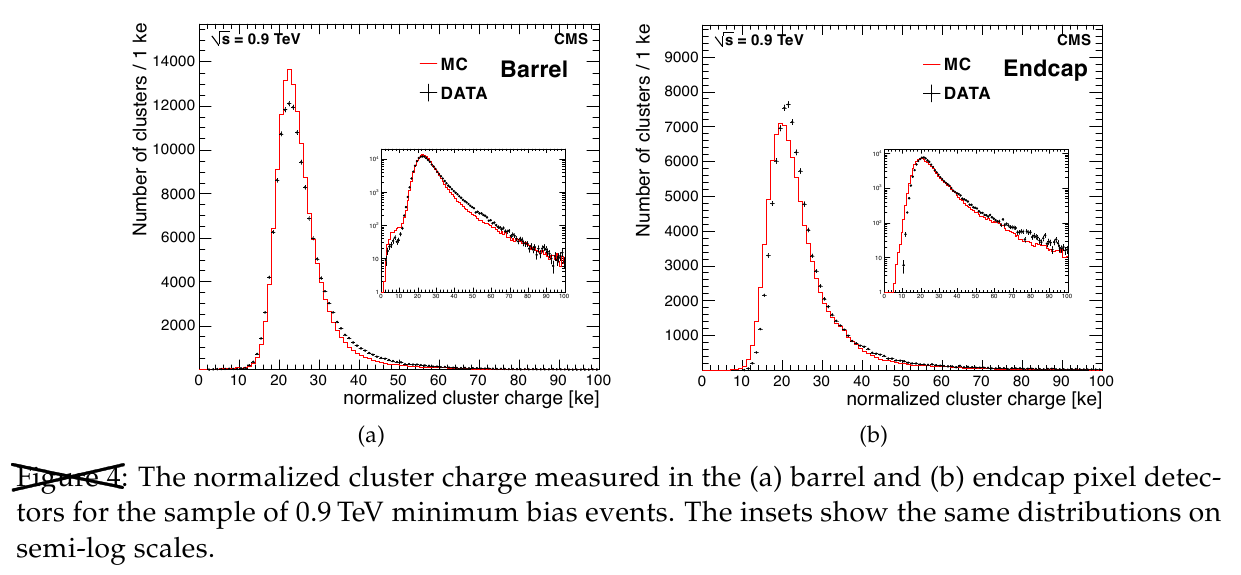
\includegraphics[width=\linewidth]{cluster_charge.png}
\end{center}
\end{frame}

\begin{frame}
\frametitle{Accuracy of the Monte Carlo}
\label{page:tracking_datamc}

\begin{itemize}
\item Also from the Tracker DPG paper
\begin{itemize}
\item high-level quantities that we apply cuts to

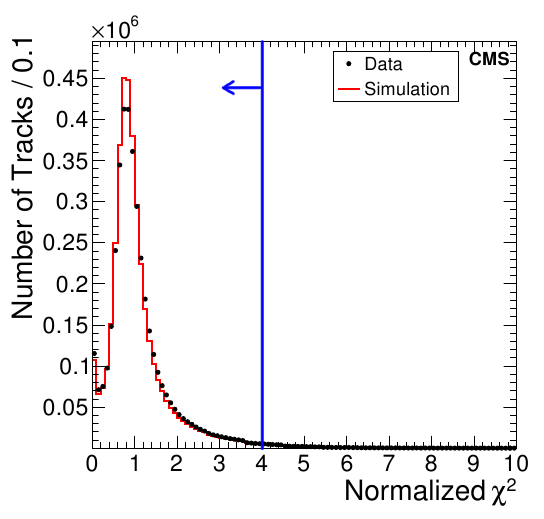
\includegraphics[width=0.5\linewidth]{normalized_chi2.png}
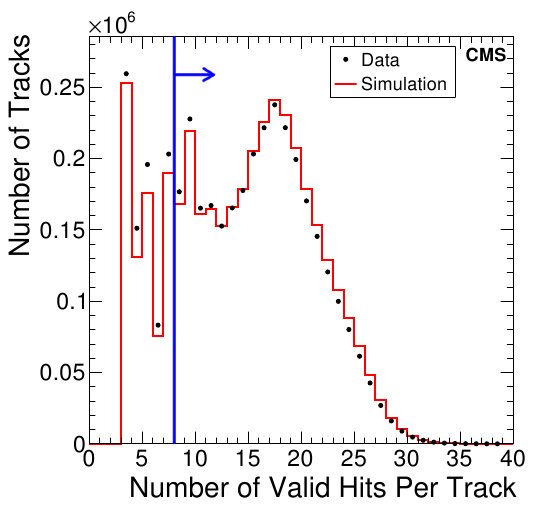
\includegraphics[width=0.5\linewidth]{number_of_hits.png}
\end{itemize}

\item Non-quantitative argument: low and high-level tracking
  distributions are well-modeled by Monte Carlo; our low-mass,
  high-$p_T$ signal differs only in geometry--- hard to imagine more
  than few-\% disagreement

\item In the following slides, we perform an explicit test to make
  this intuition more precise
\end{itemize}
\end{frame}

\begin{frame}
\frametitle{$\phi(1020)$ resonance study}
\label{page:phi_study}

Data/MC comparisons of ``close-by muons'' in our sample ($\Delta R \sim 0.1$)

\begin{columns}
\column{0.5\linewidth}

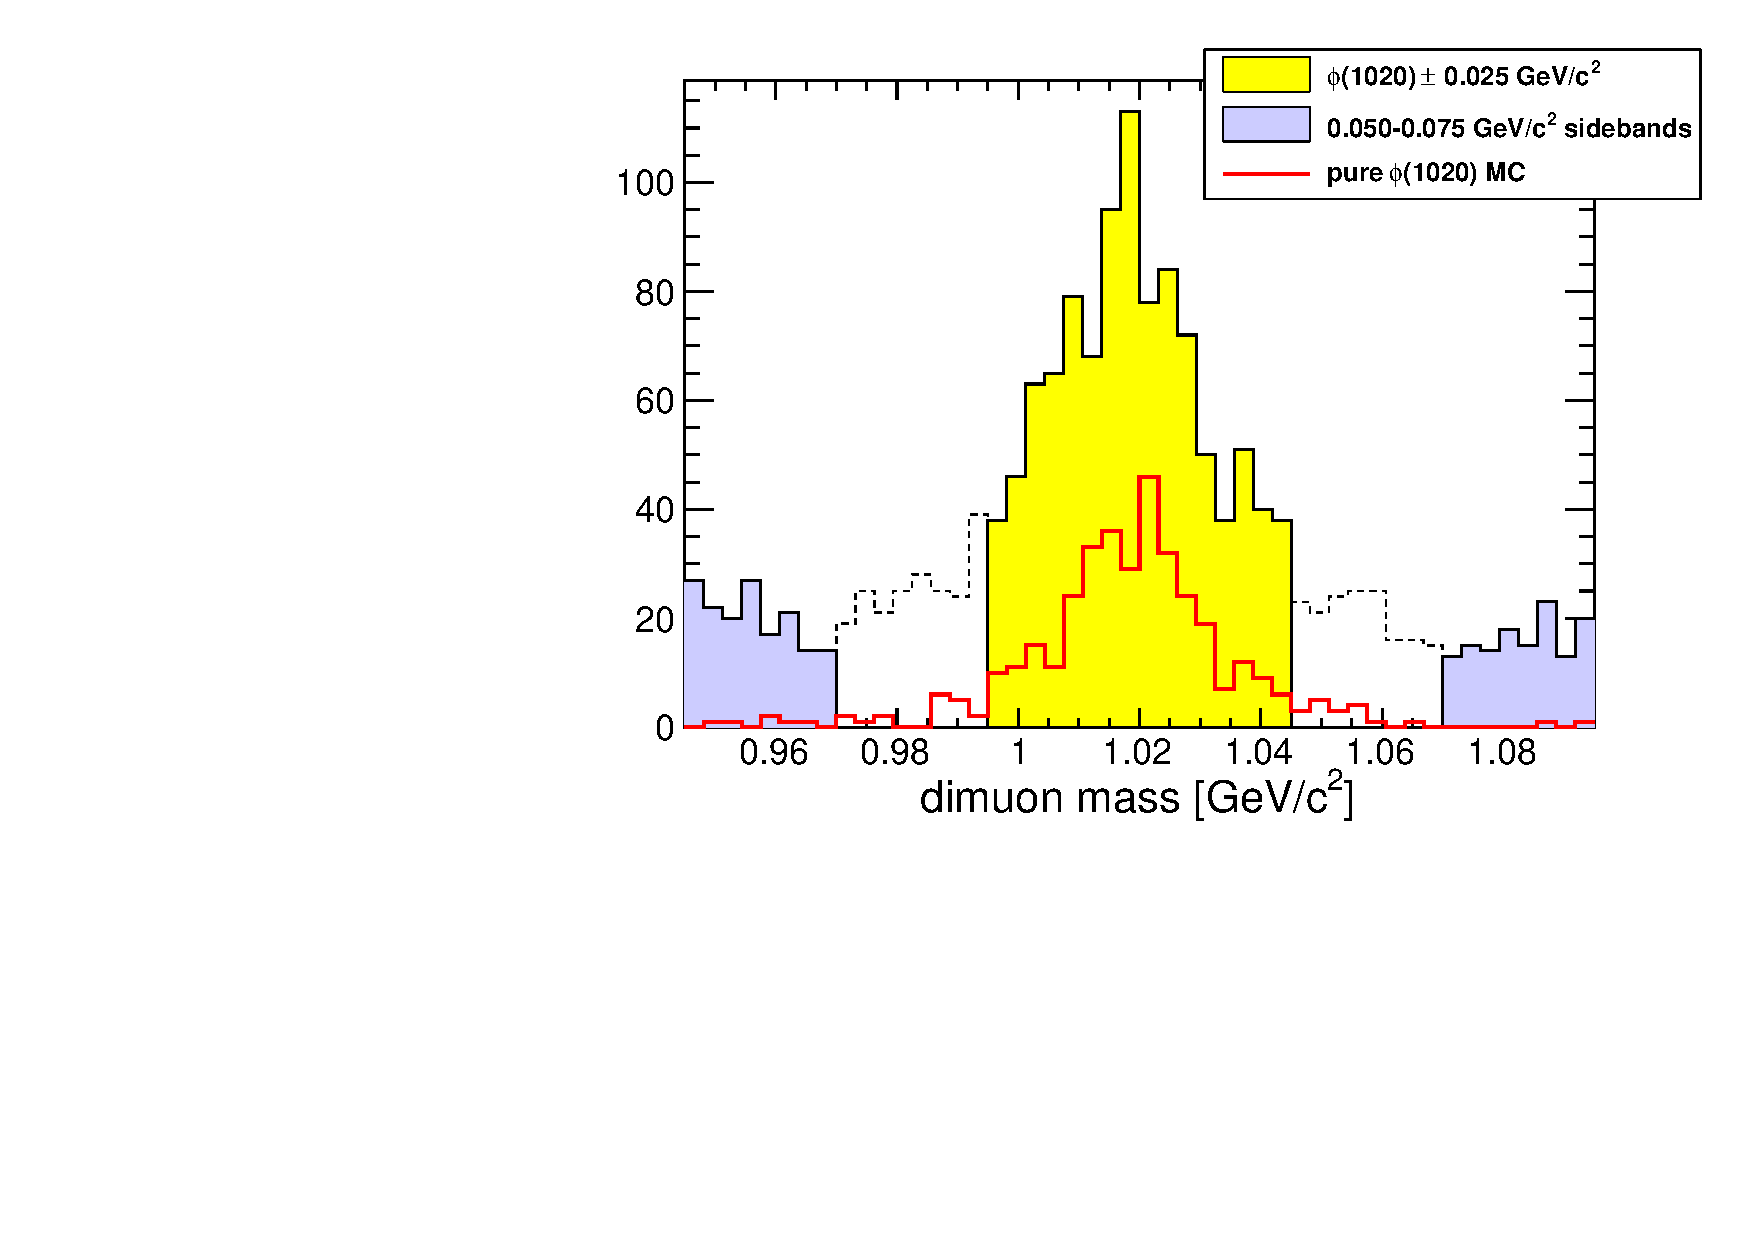
\includegraphics[width=\linewidth]{phi_mass.pdf}

\column{0.5\linewidth}
\begin{itemize}
\item Compare data and MC distributions of the $\phi(1020)$
\begin{itemize}
\item exactly two muons/event
\item prompt ($L_{xy} < 1$~mm)
\item in jets ($Iso > 3$~GeV/$c$)
\item one muon $p_T > 10$~GeV/$c$
\item sideband-subtracted data, normalized MC
\end{itemize}
\end{itemize}
\end{columns}

\vspace{0.25 cm}
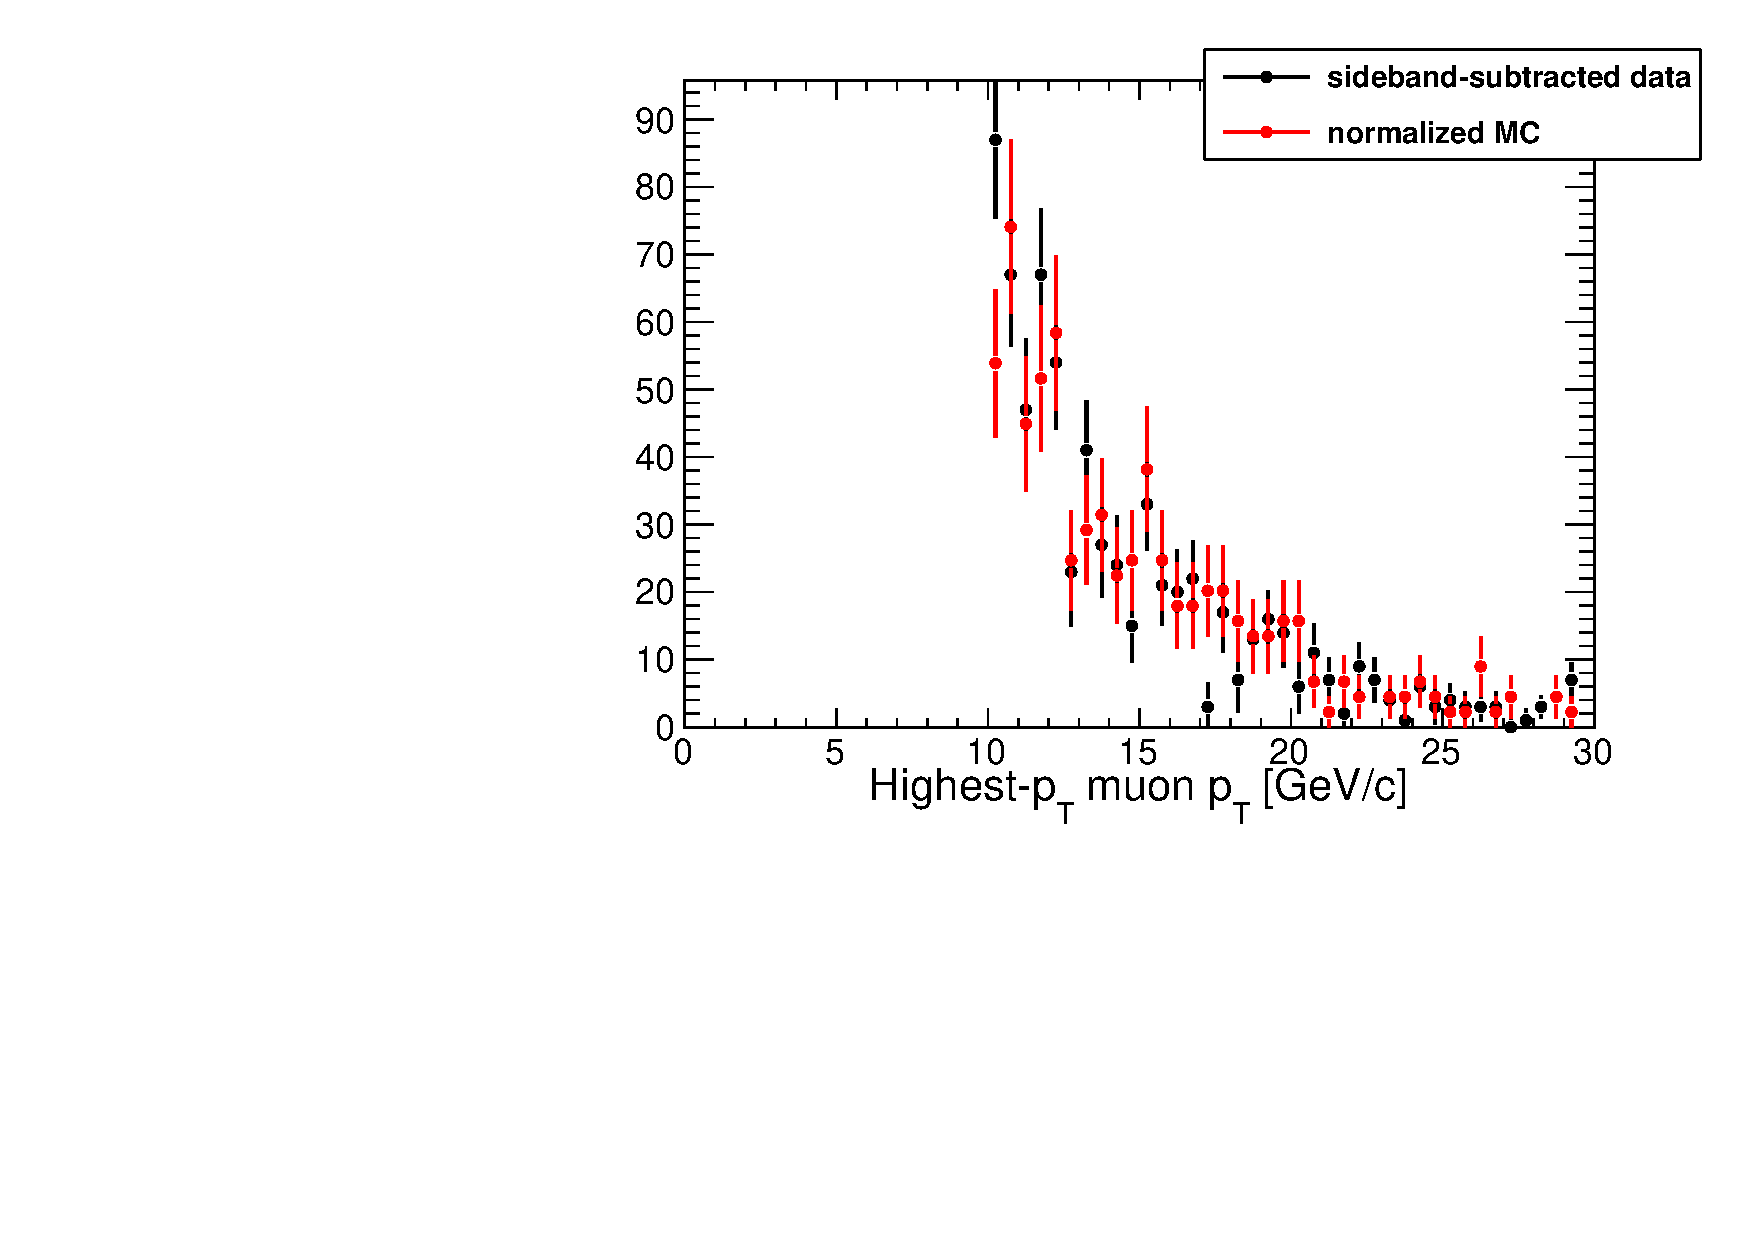
\includegraphics[width=0.5\linewidth]{phi_muon1pt.pdf}
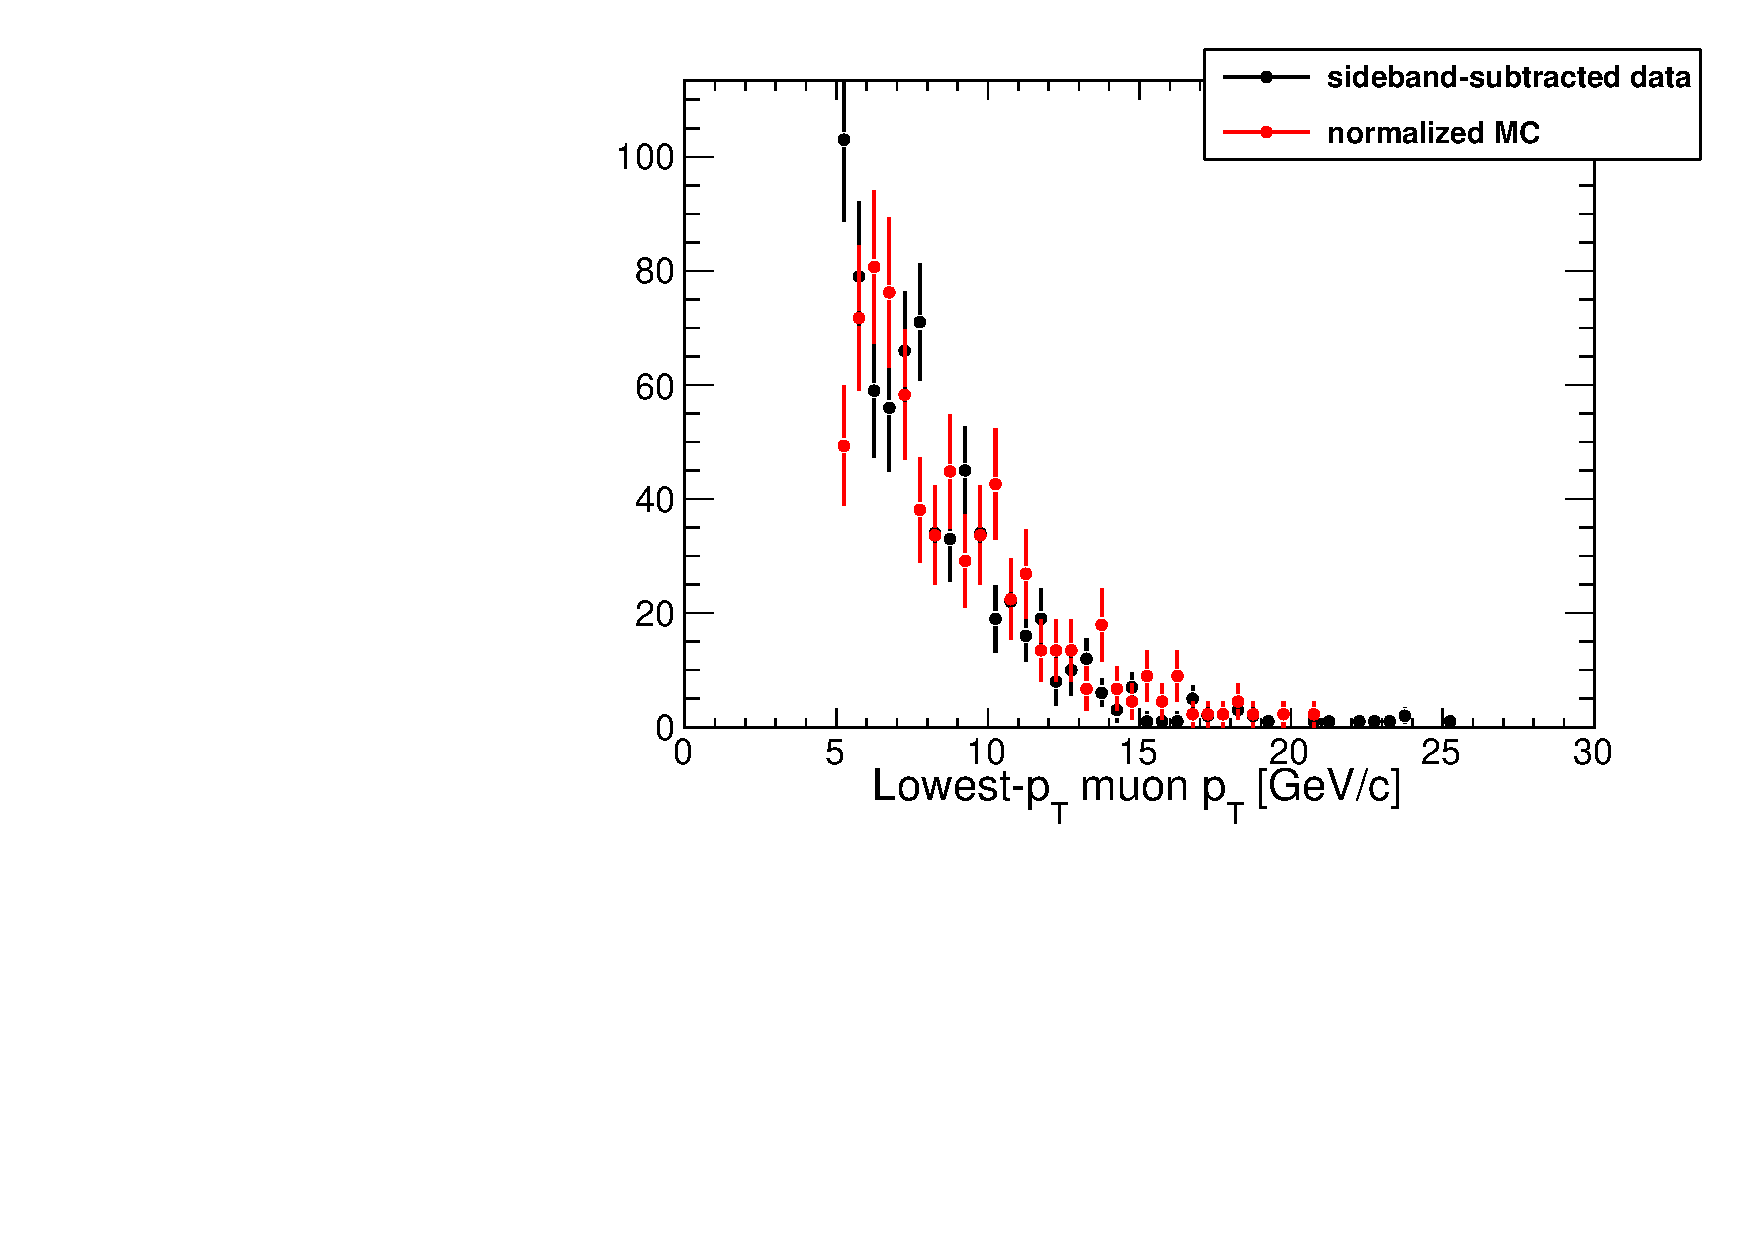
\includegraphics[width=0.5\linewidth]{phi_muon2pt.pdf}
\end{frame}

\begin{frame}
\frametitle{$\phi(1020)$ resonance study}

Track quality cuts:

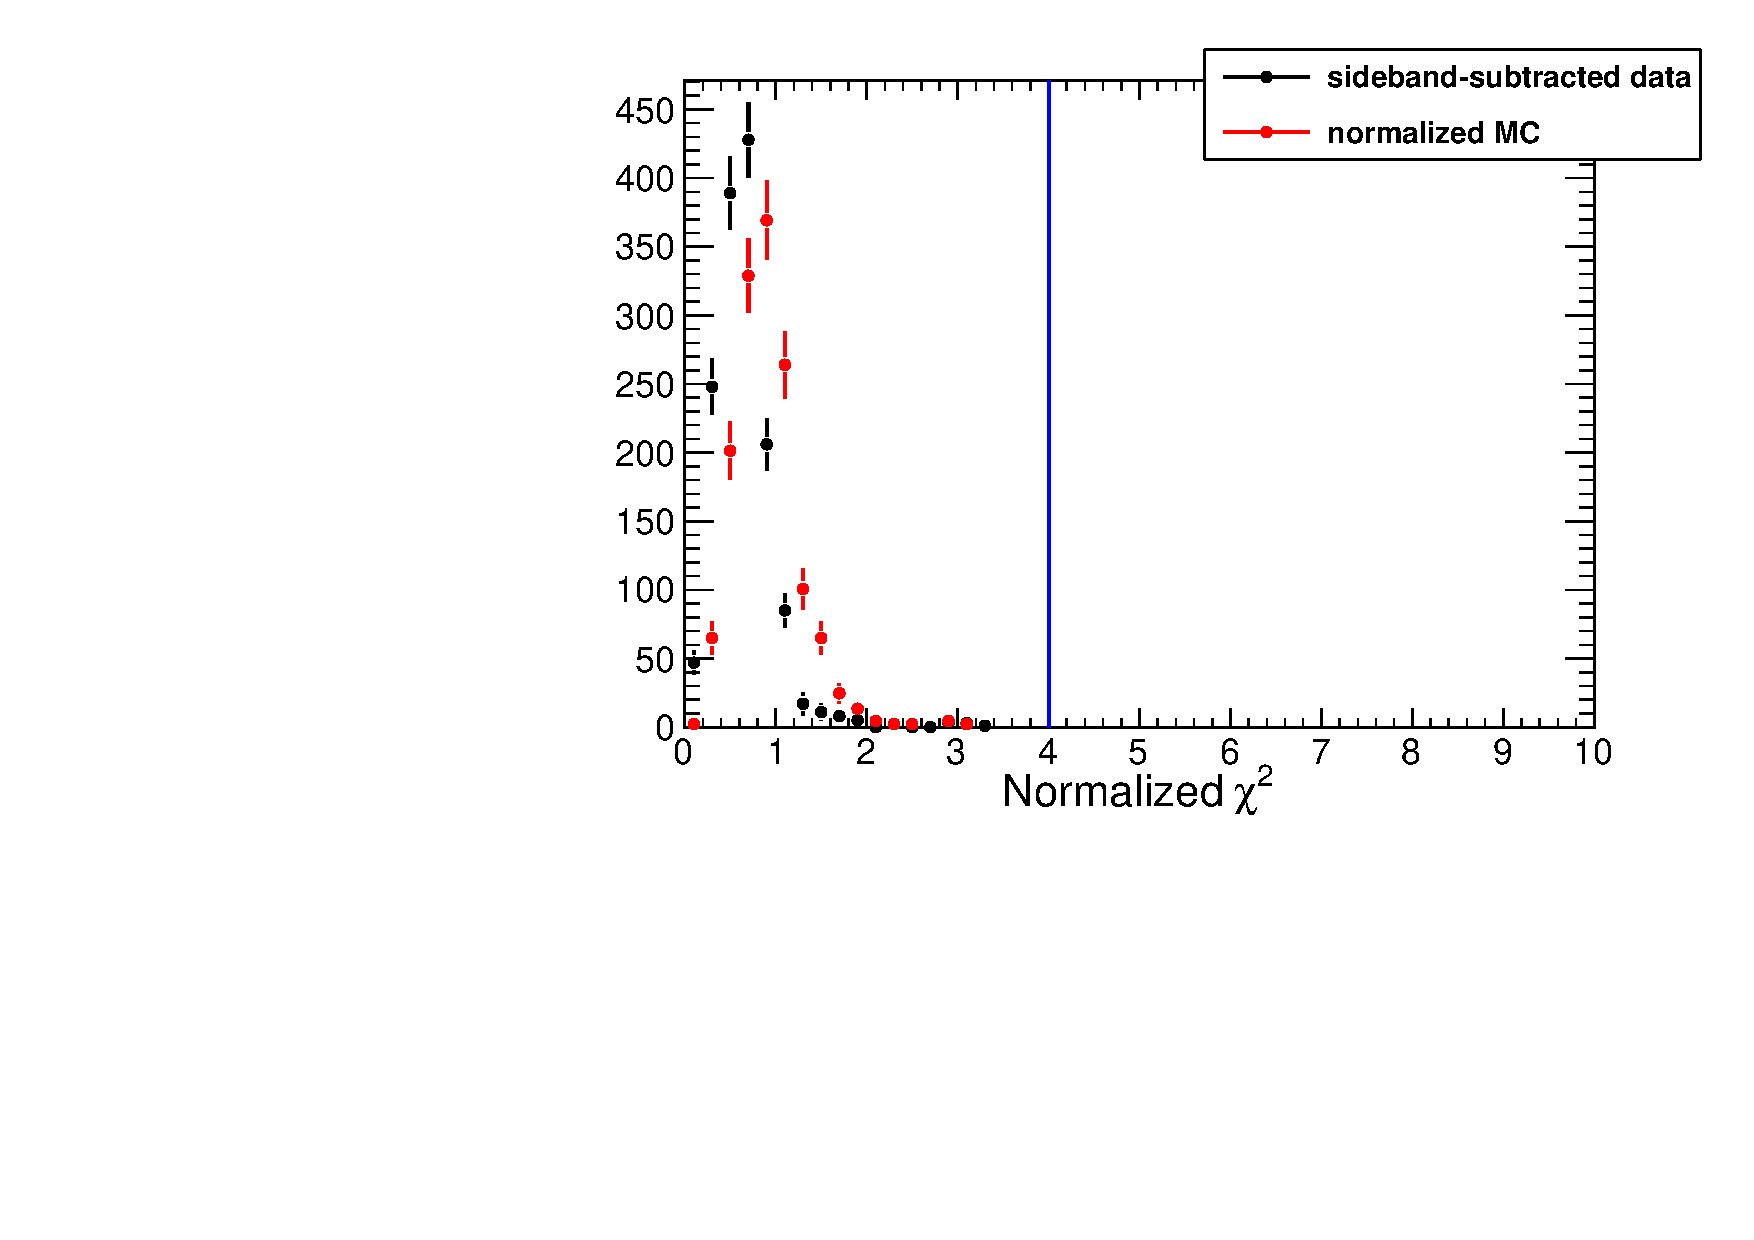
\includegraphics[width=0.5\linewidth]{phi_normchi2.pdf}
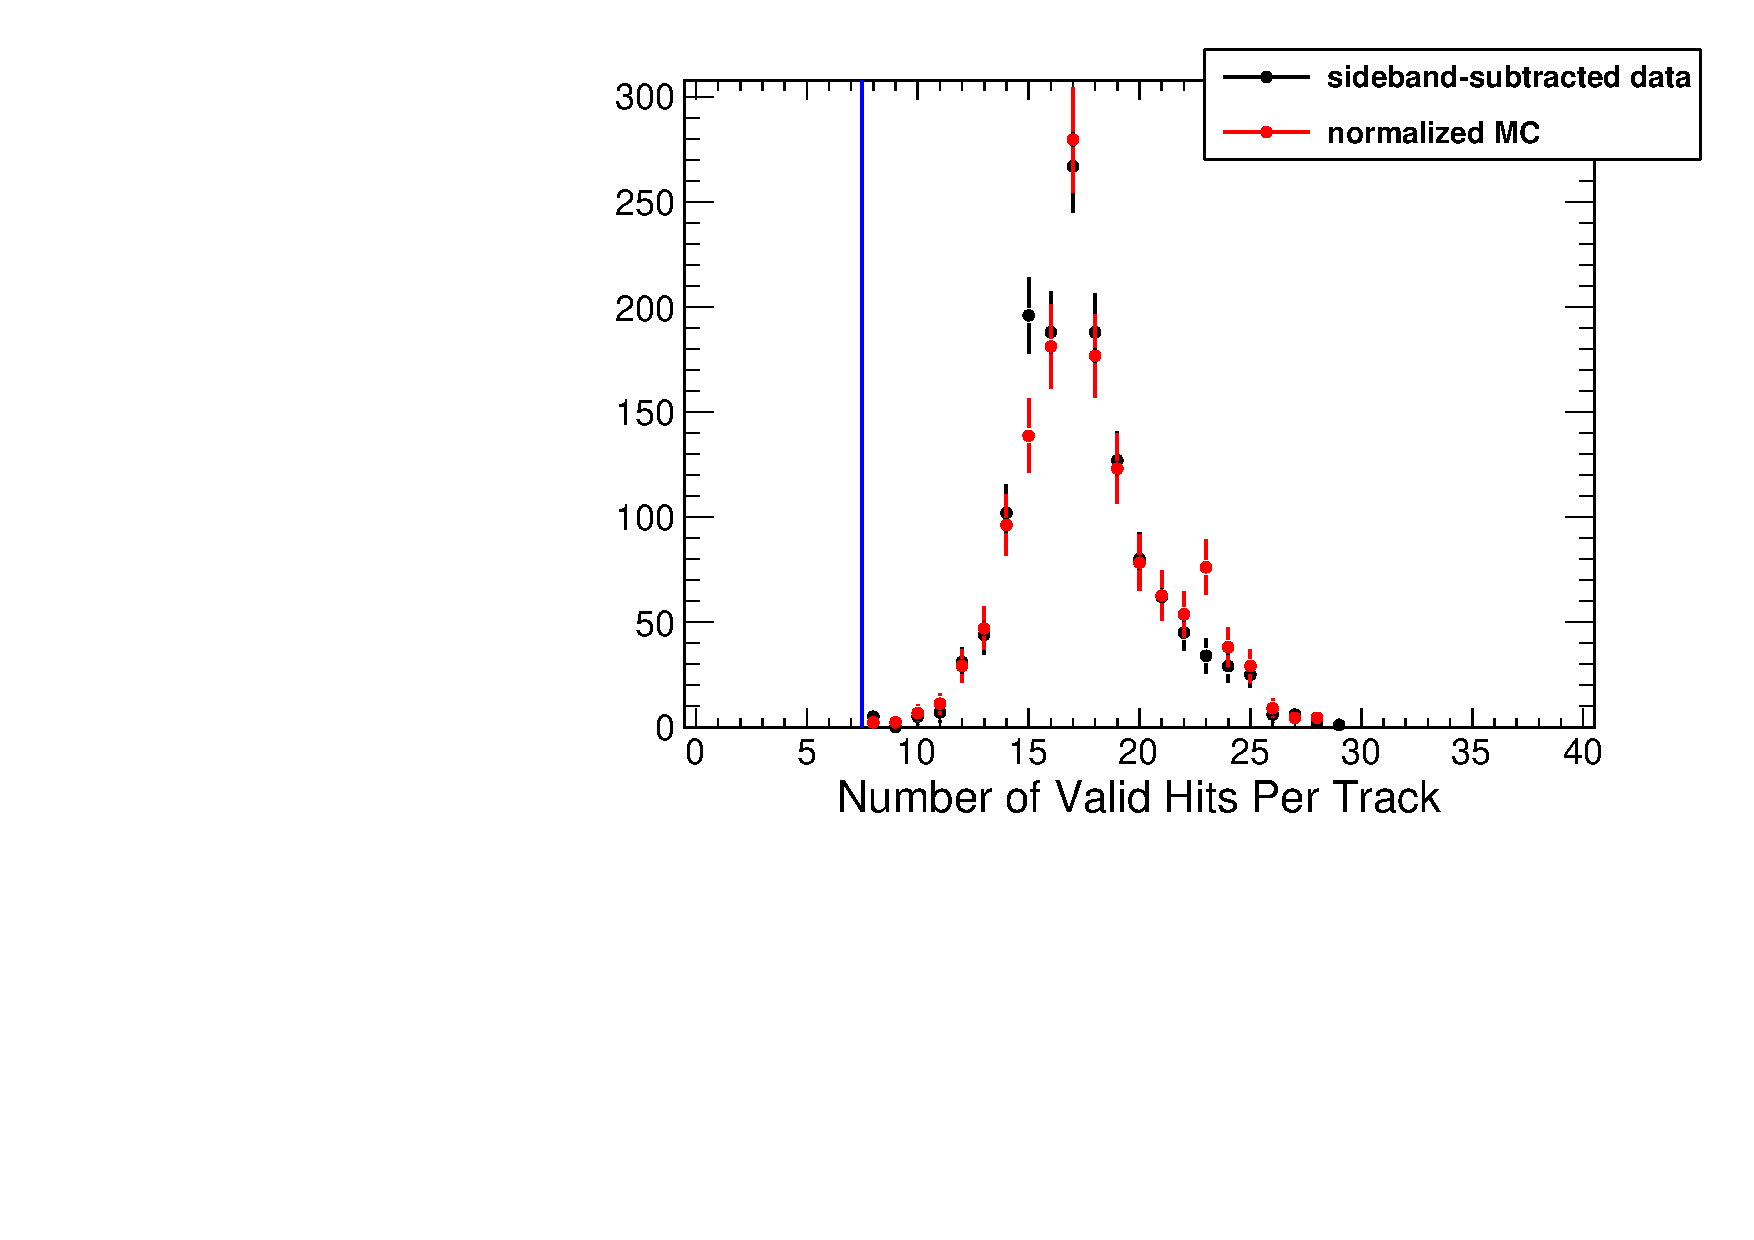
\includegraphics[width=0.5\linewidth]{phi_hits.pdf}

\vspace{0.25 cm}
Muon quality cuts:

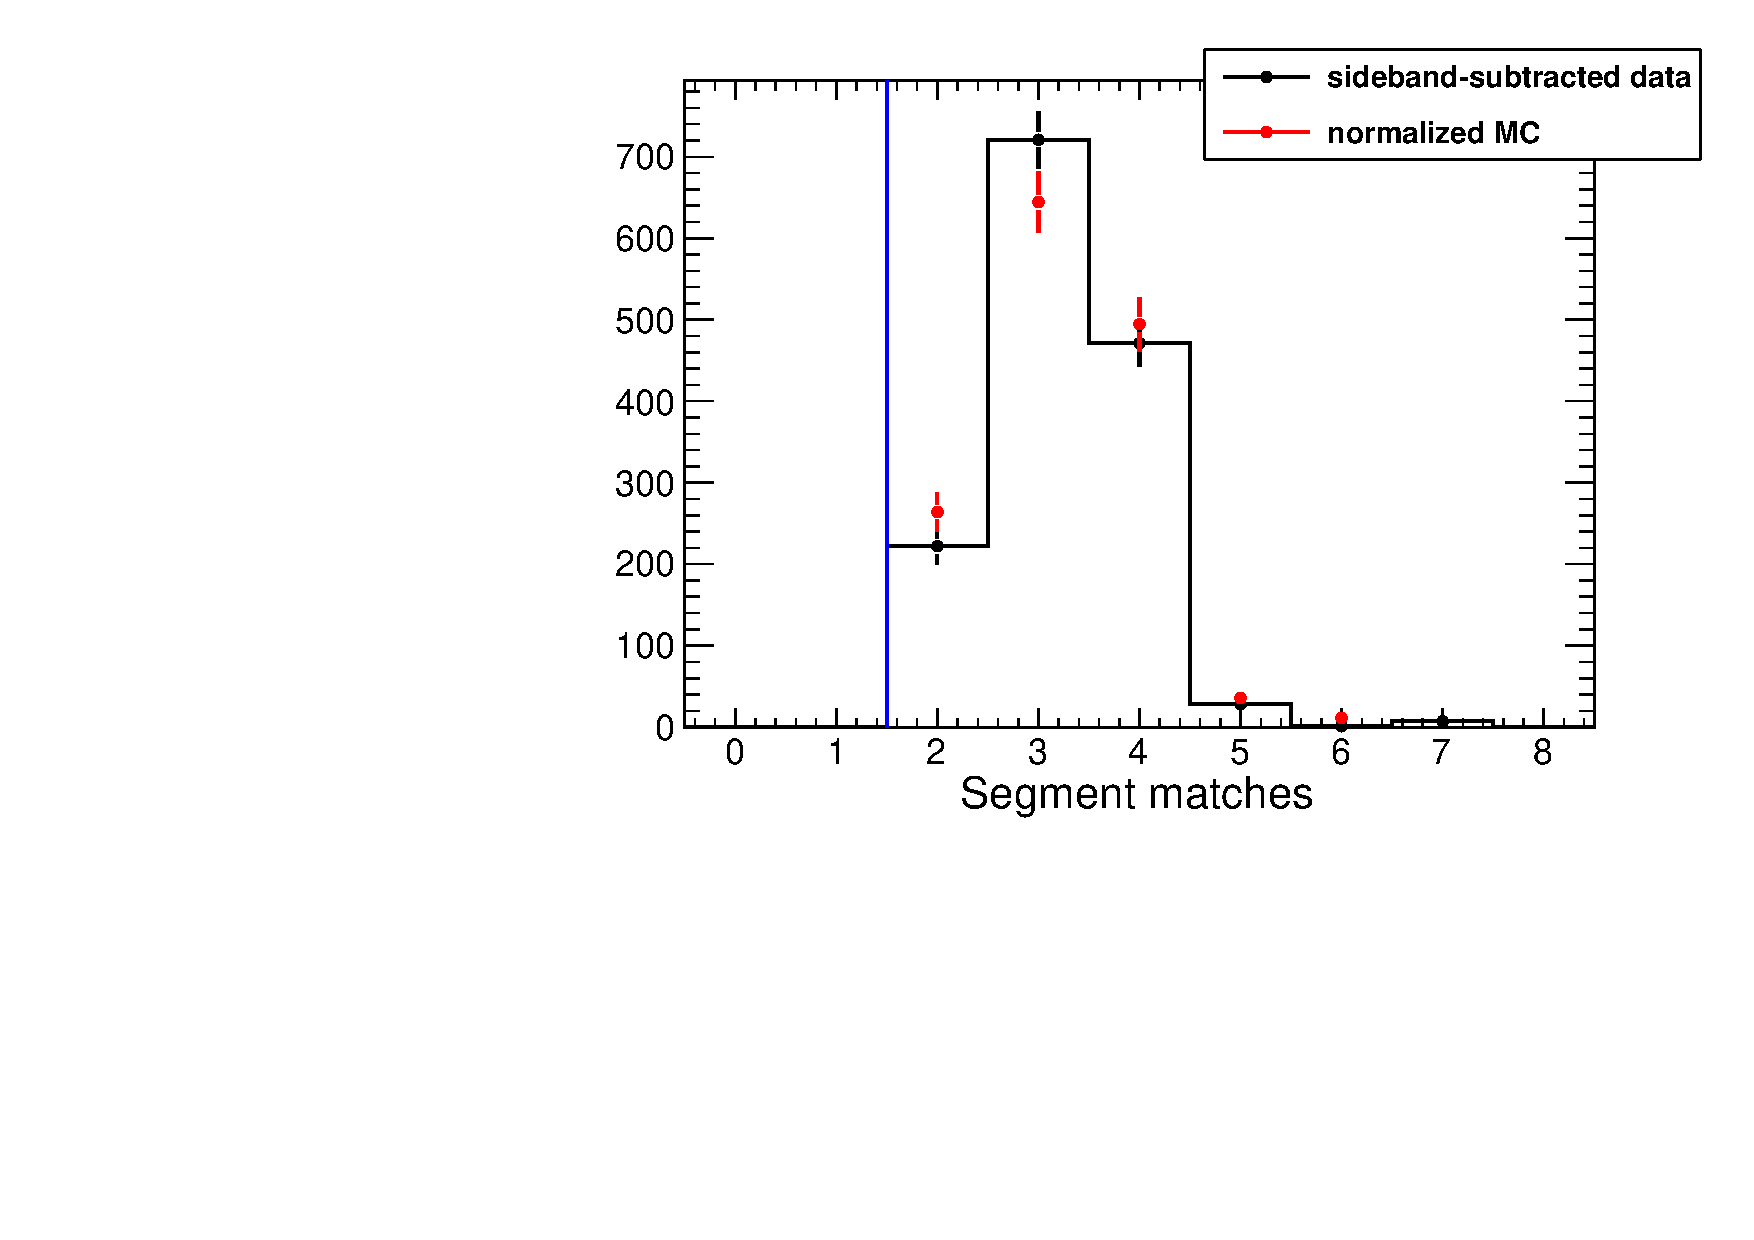
\includegraphics[width=0.5\linewidth]{phi_matches.pdf}

\vspace{-3.5 cm}
\hfill \begin{minipage}{0.45\linewidth}
\scriptsize
``Normalized $\chi^2$'' and ``Number of Valid Hits Per Track'' are the
same as page~\pageref{page:tracking_datamc}, but for our muons ($p_T >
5$~GeV/$c$), cuts are far from bulk of distribution

\vspace{0.25 cm}
MC has STARTUP conditions applied

\vspace{0.25 cm}
Comparisons made after all cuts
\end{minipage}

\vspace{2.5 cm}
\end{frame}

\begin{frame}
\frametitle{$\phi(1020)$ resonance study}

Muon residuals:

\scriptsize
\begin{itemize}
\item Relevant for number of muon segments cut (track $\to$ segment must match)
\item Muon alignment effect is negligible because of large multiple scattering
\end{itemize}

\hfill 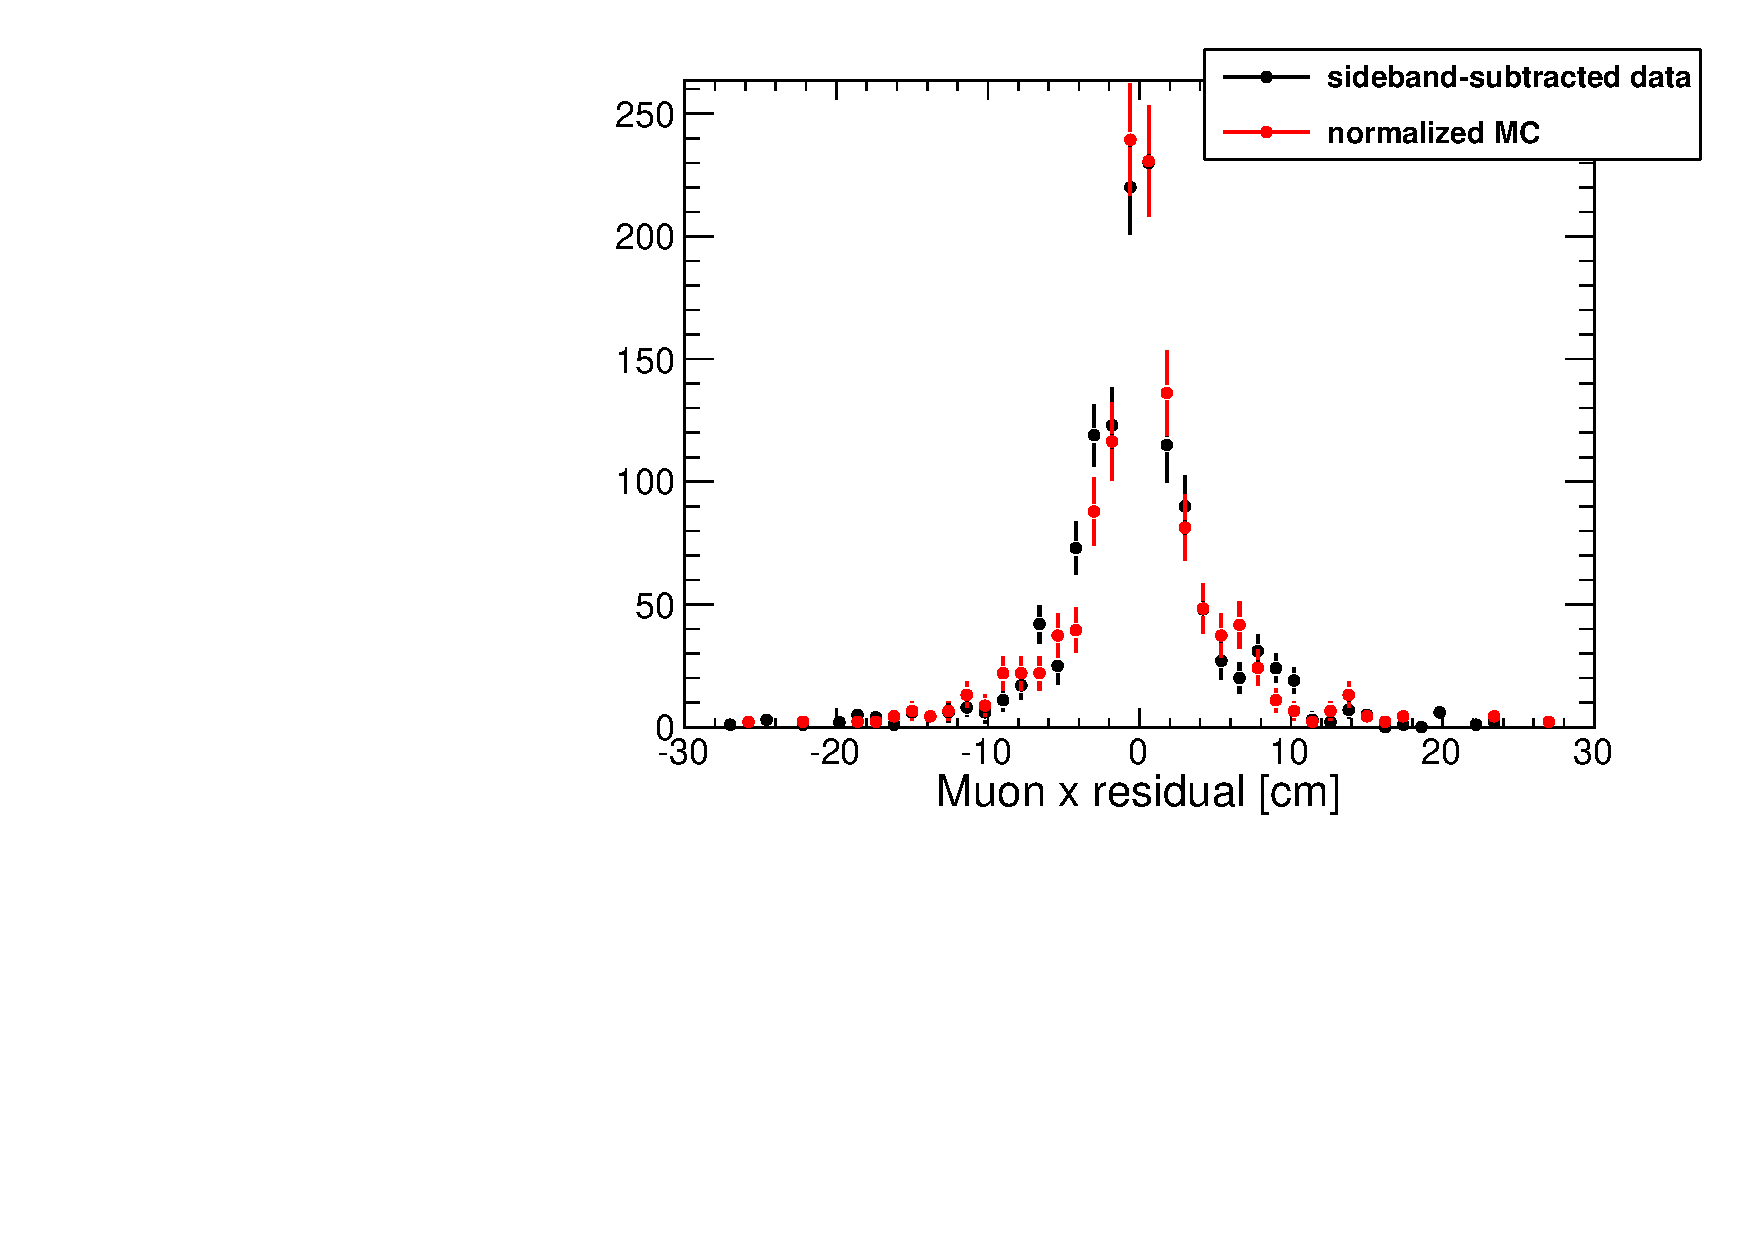
\includegraphics[width=0.45\linewidth]{phi_st1x.pdf}
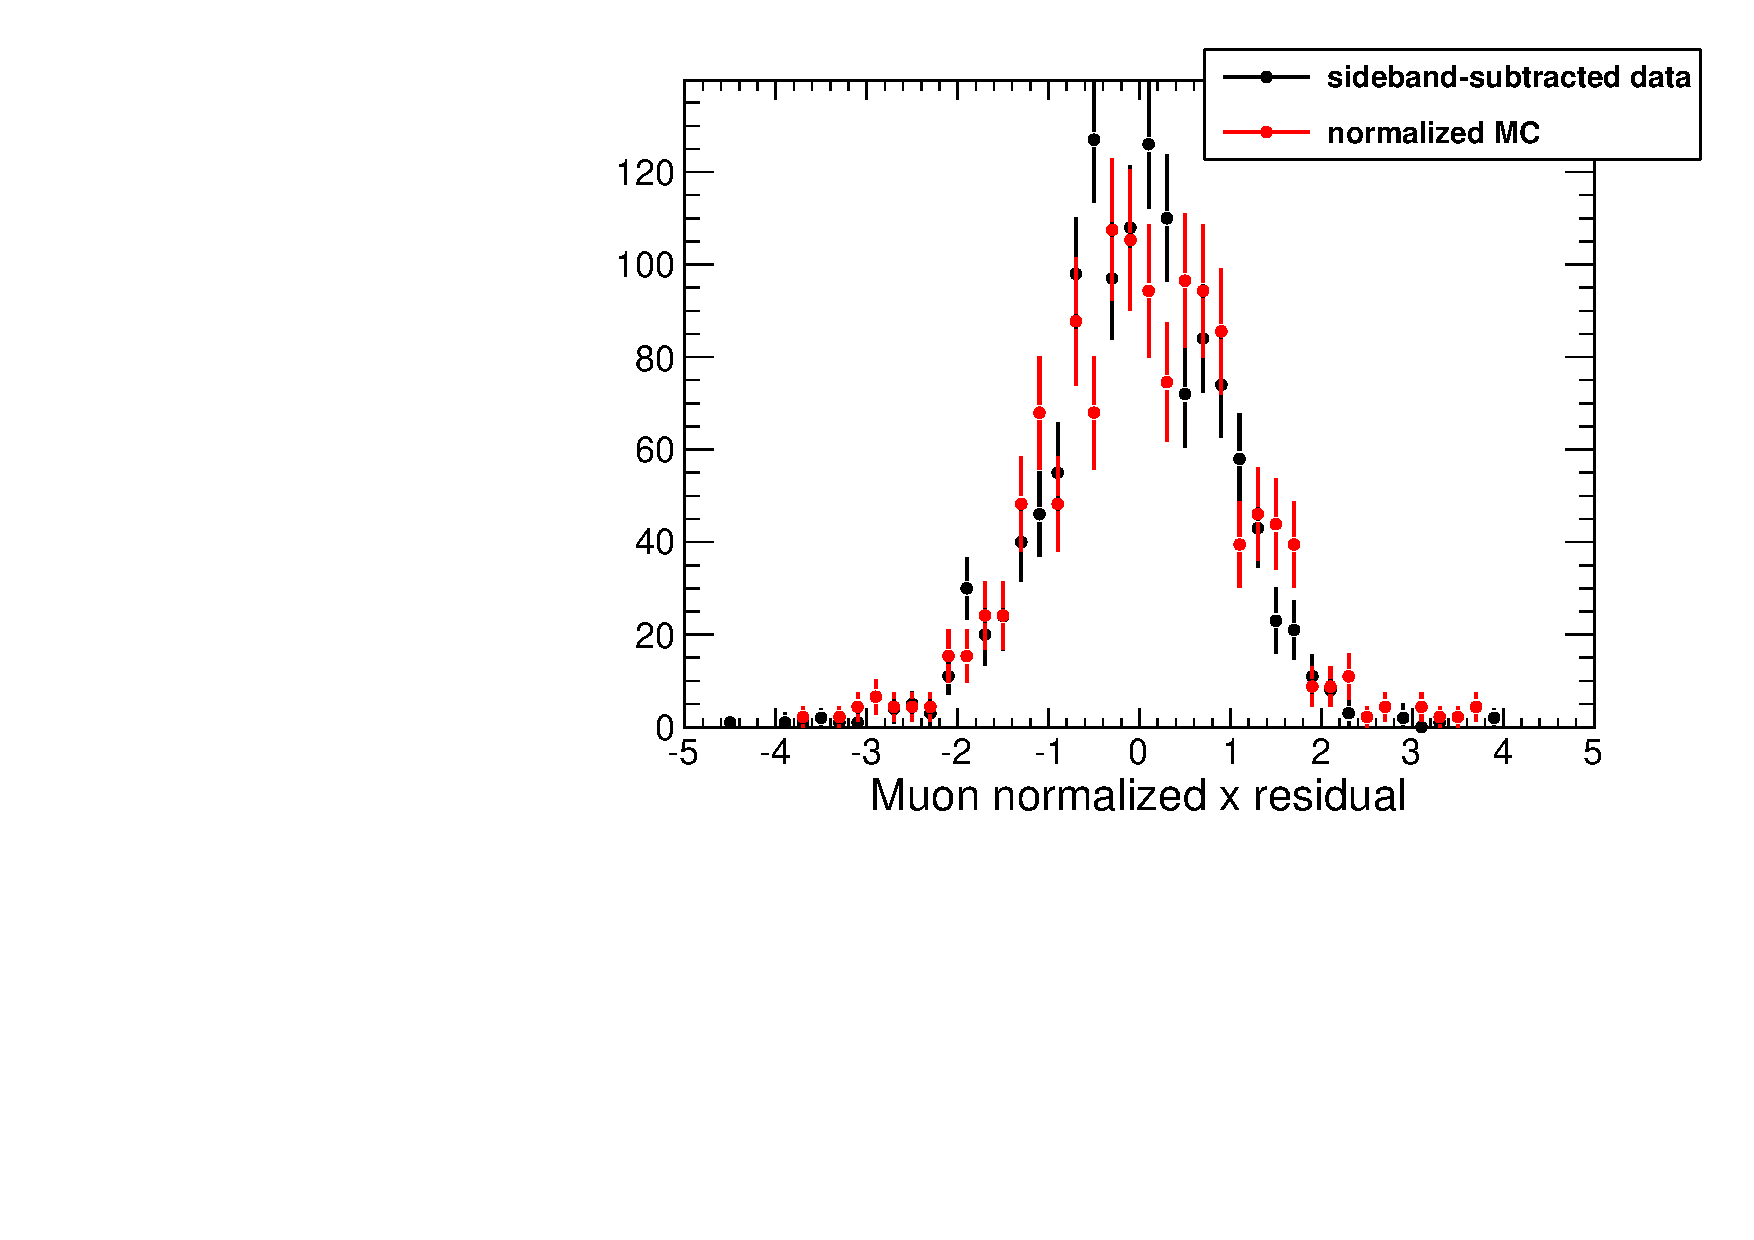
\includegraphics[width=0.45\linewidth]{phi_st1xsig.pdf}

\hfill 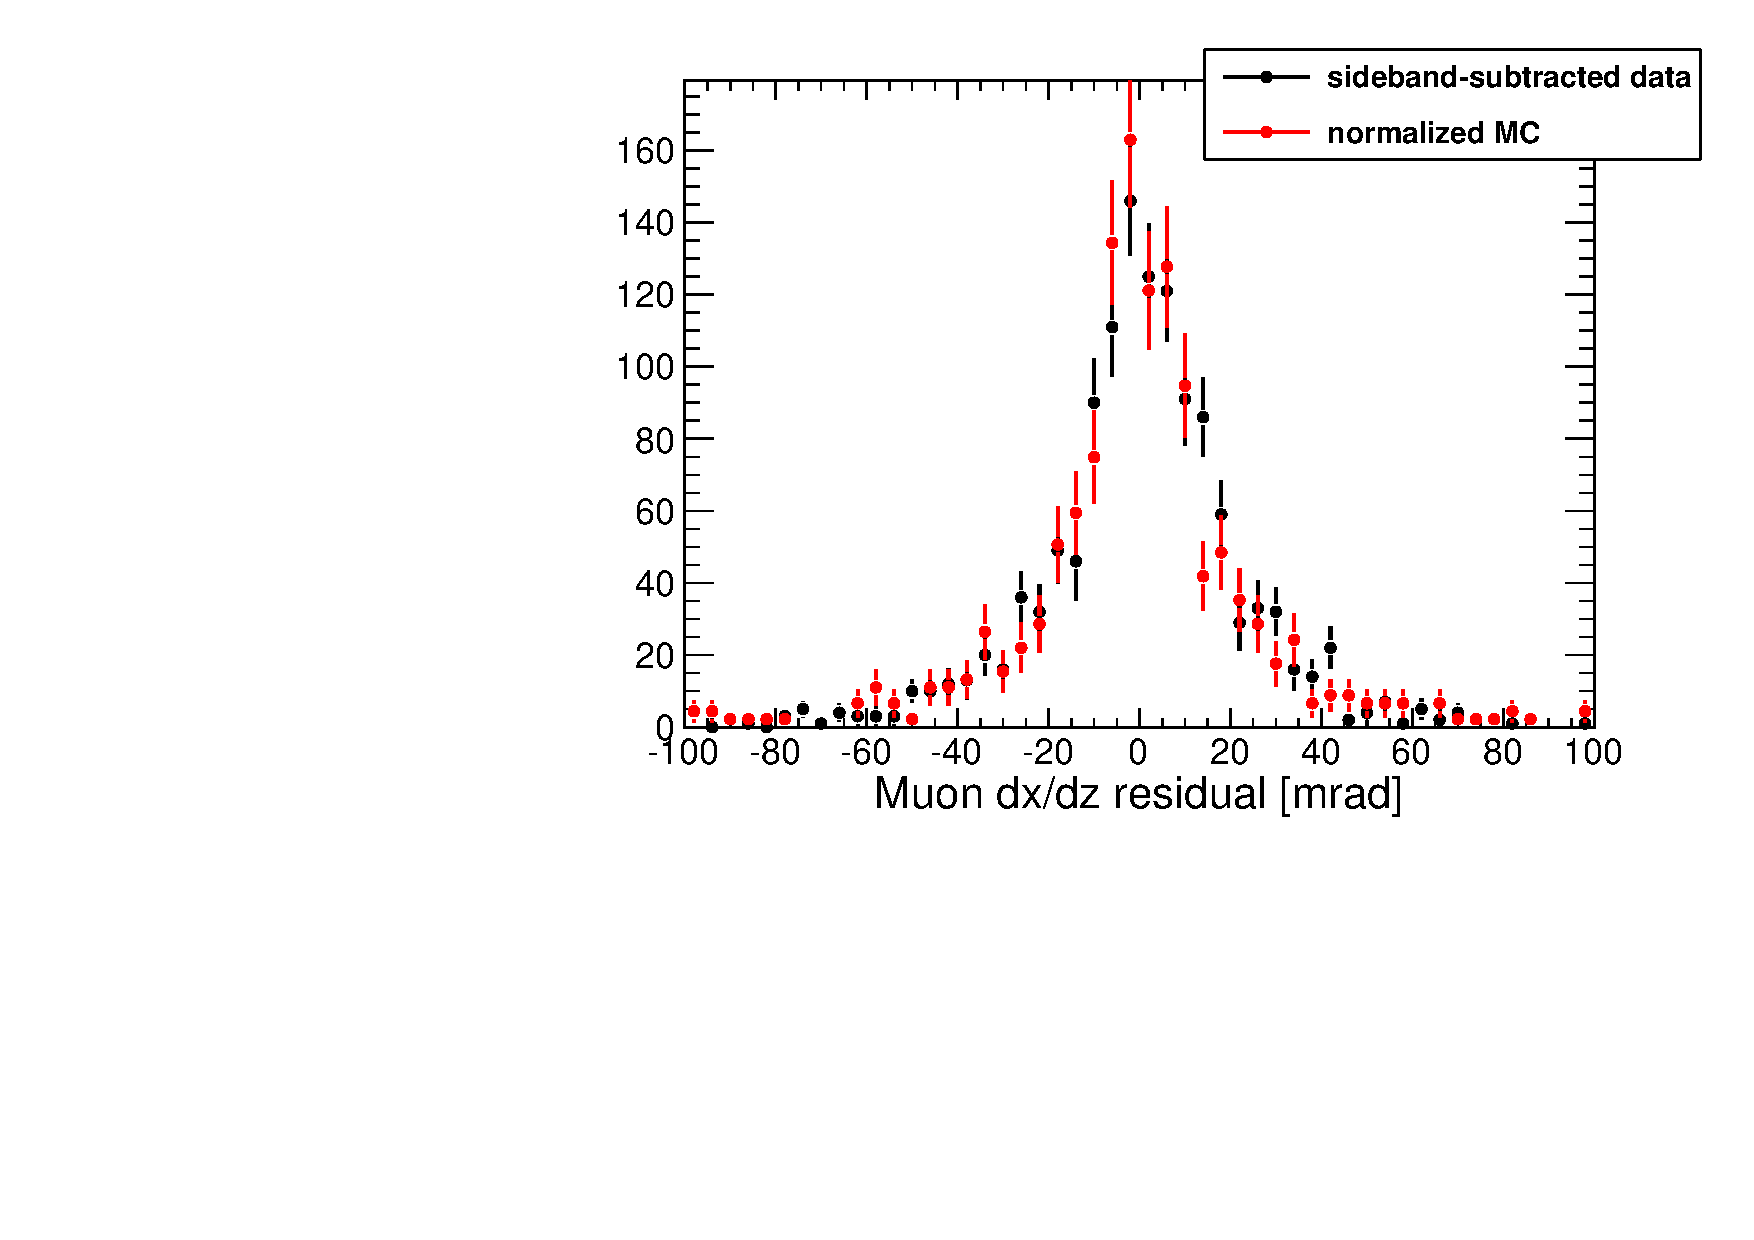
\includegraphics[width=0.45\linewidth]{phi_st1dxdz.pdf}
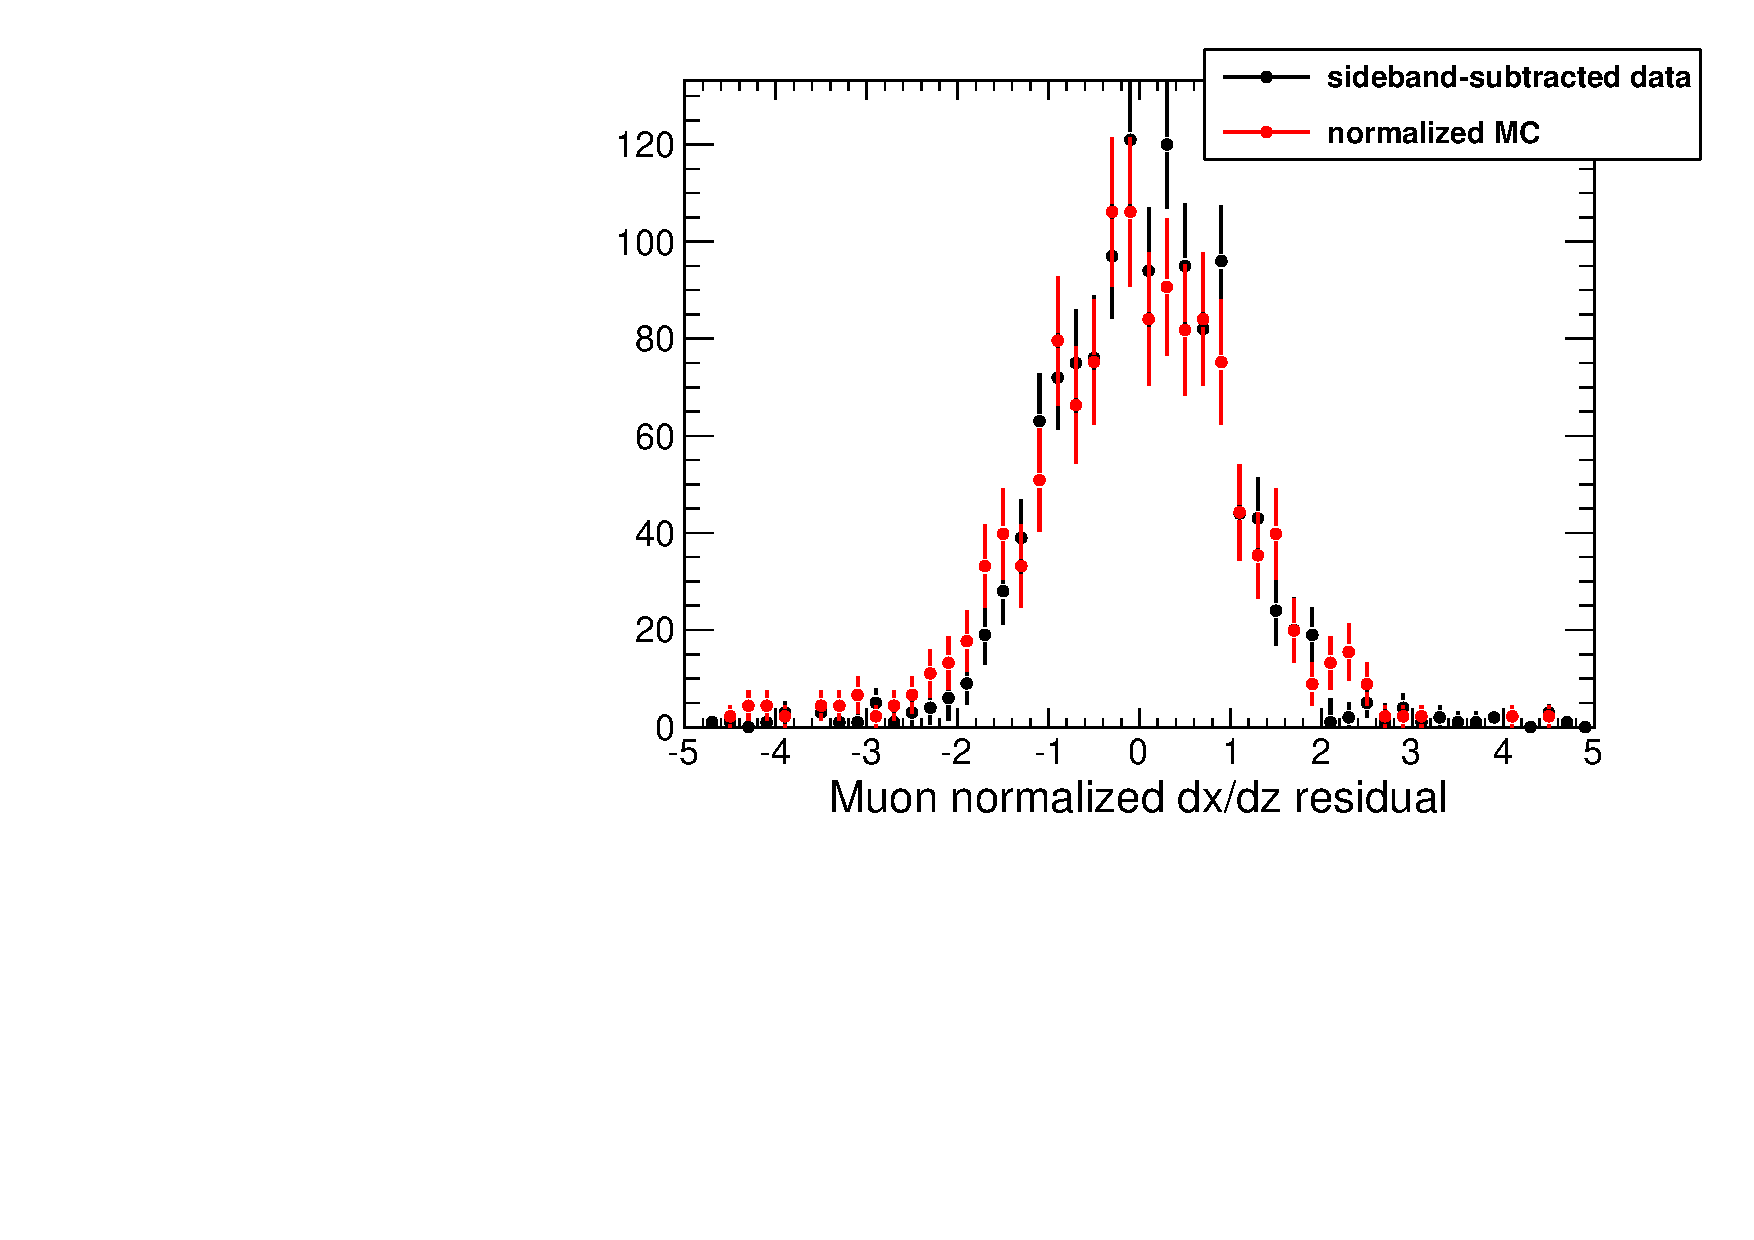
\includegraphics[width=0.45\linewidth]{phi_st1dxdzsig.pdf}
\end{frame}

\begin{frame}
\frametitle{$\phi(1020)$ resonance study}

Additional comparisons:

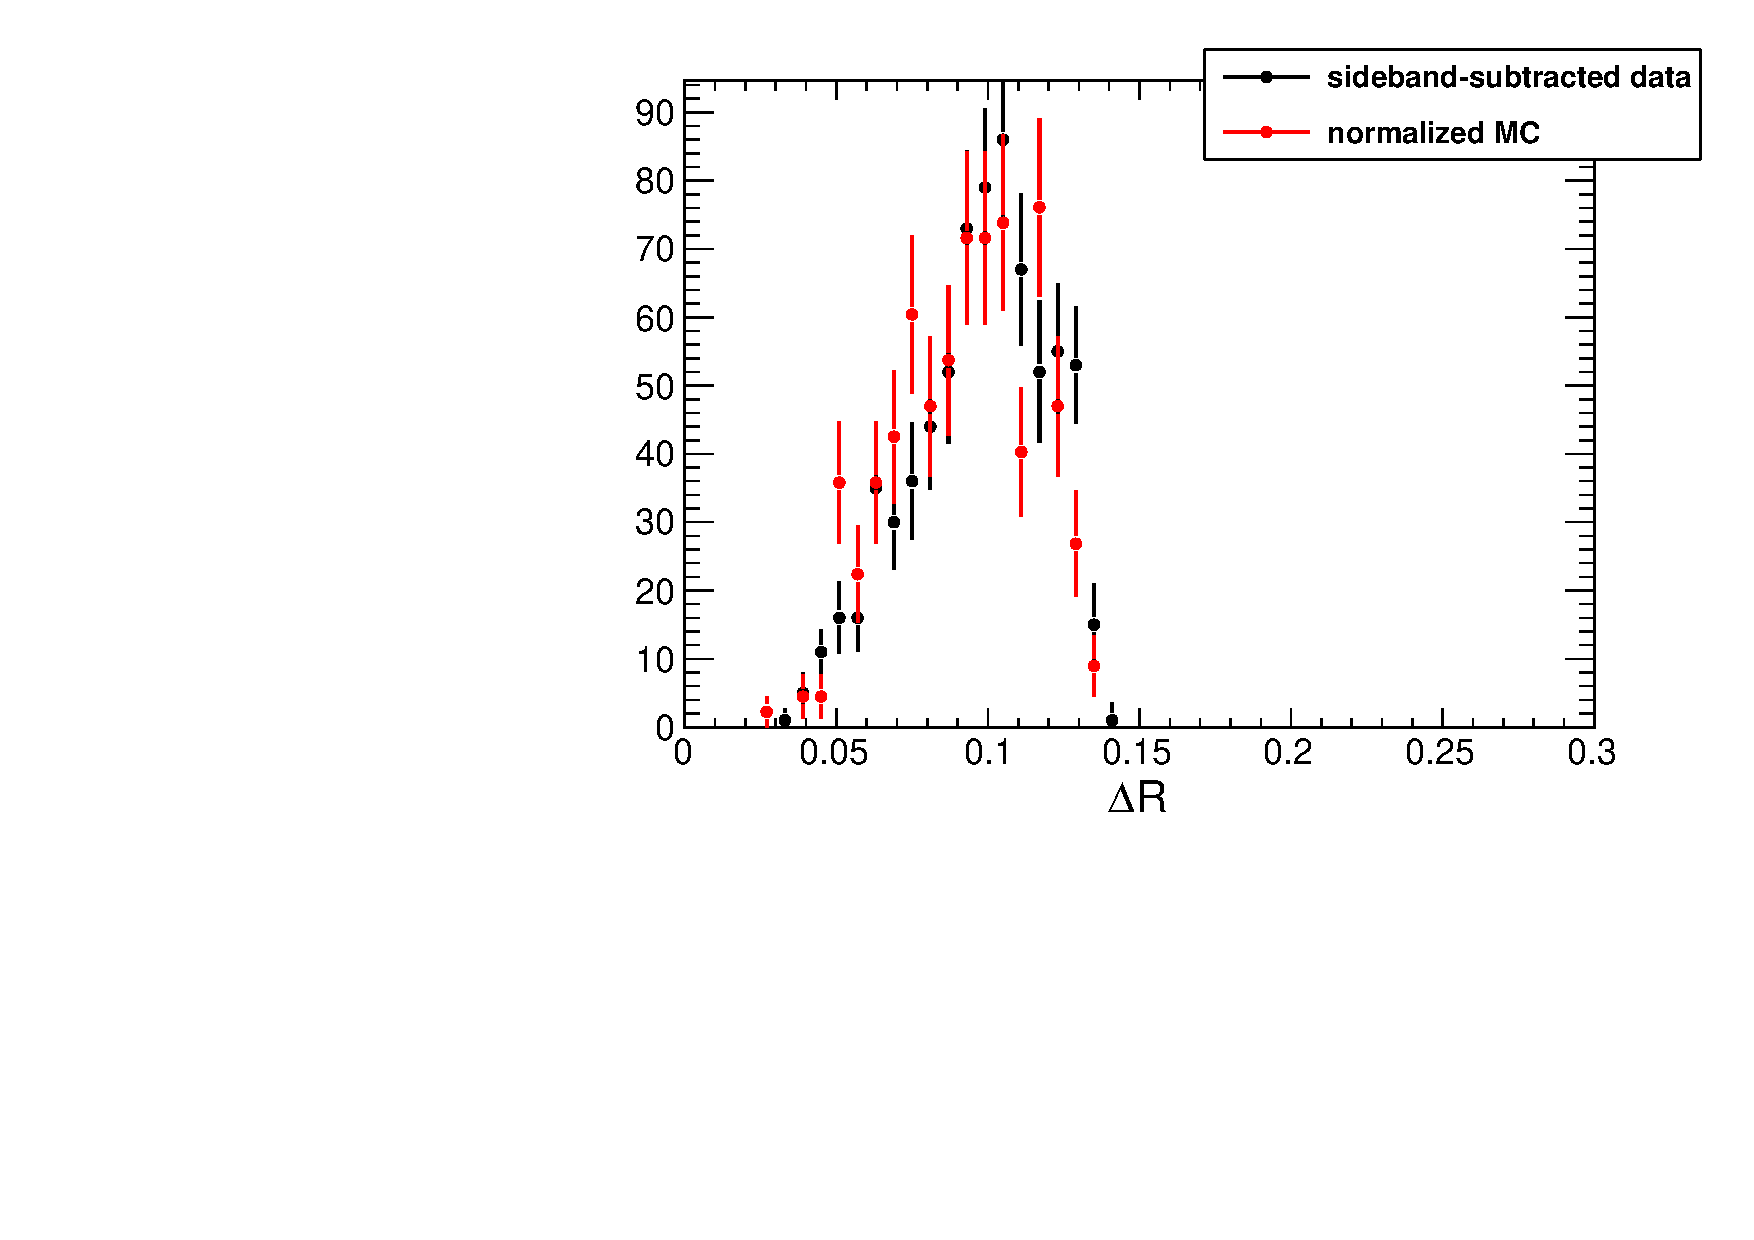
\includegraphics[width=0.45\linewidth]{phi_dr.pdf}
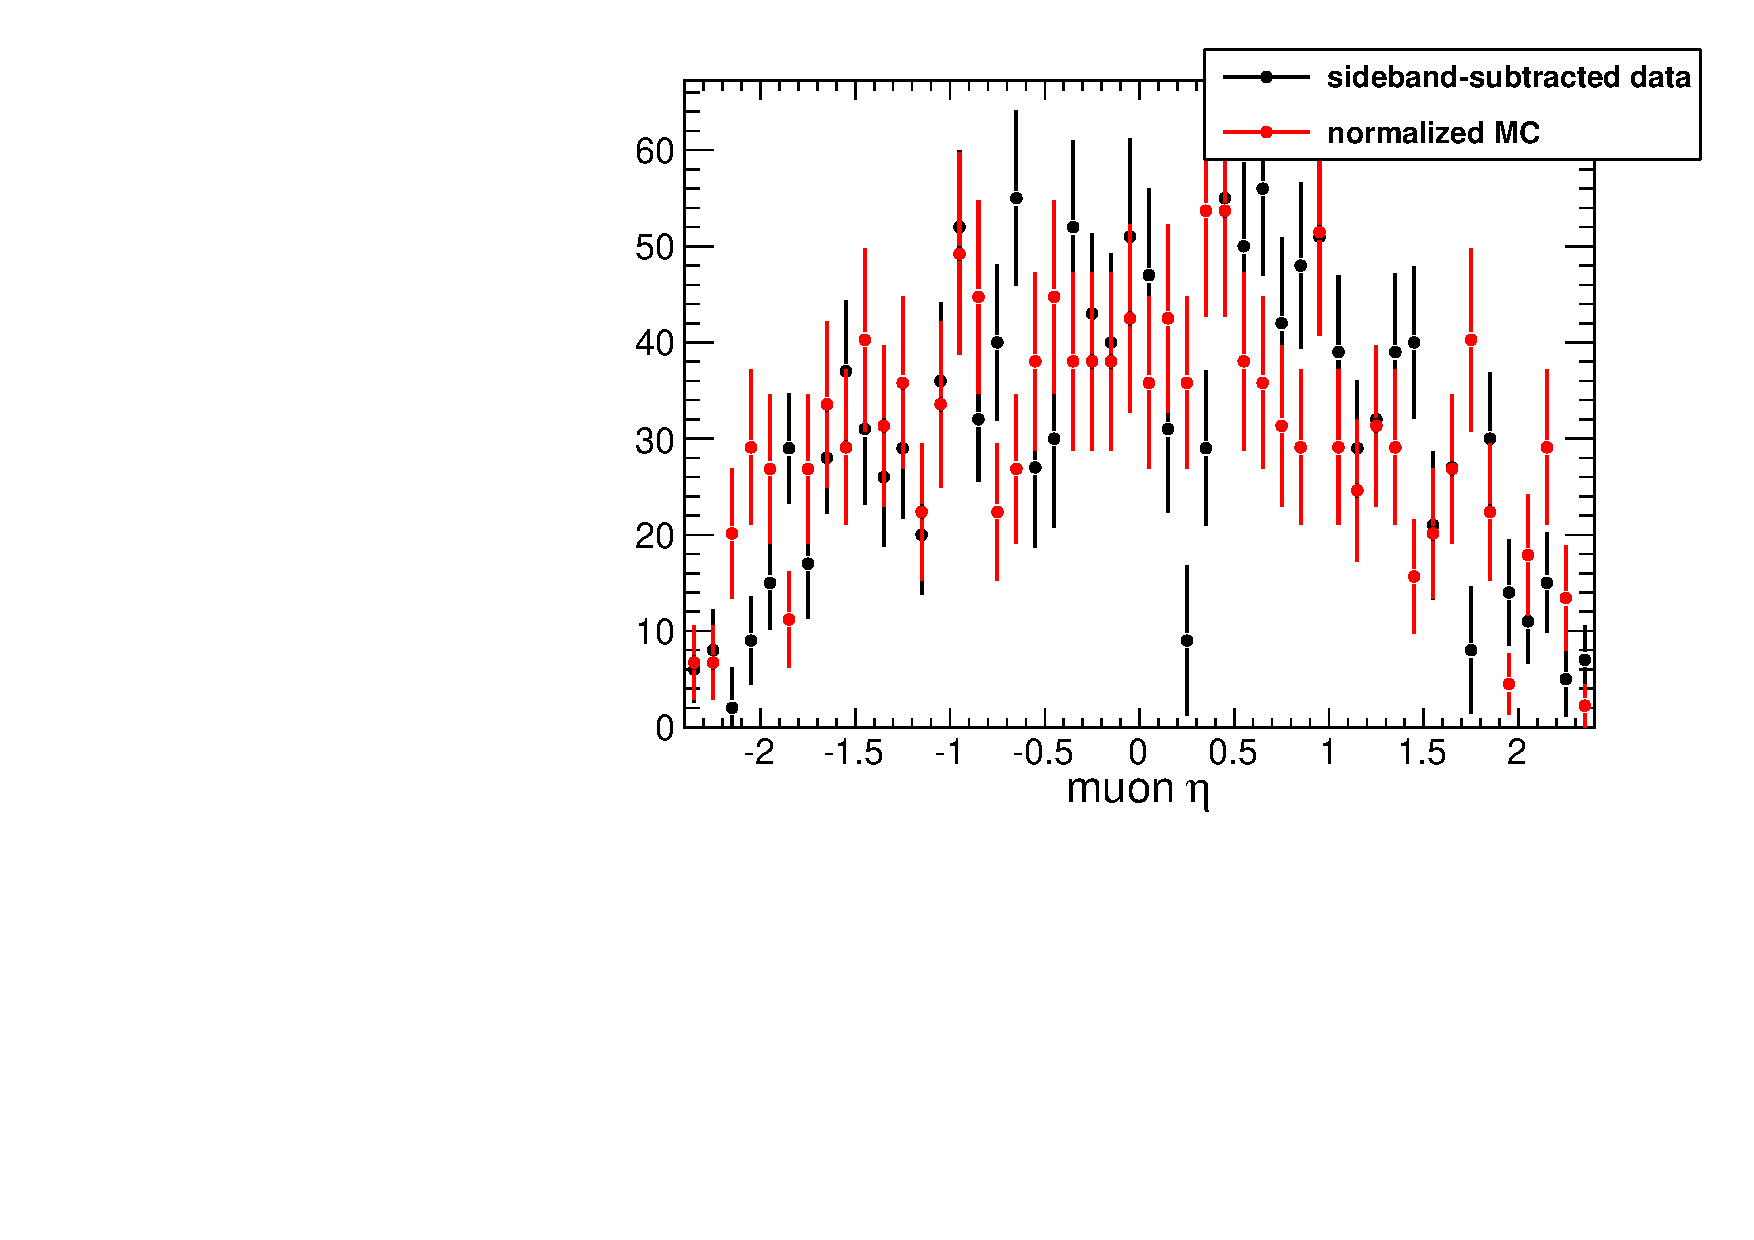
\includegraphics[width=0.45\linewidth]{phi_eta.pdf}

Cuts used to define this sample {\scriptsize (so that data and MC would have the
same production mechanism: $\phi(1020)$ in light quark jets)}:

\vspace{0.25 cm}
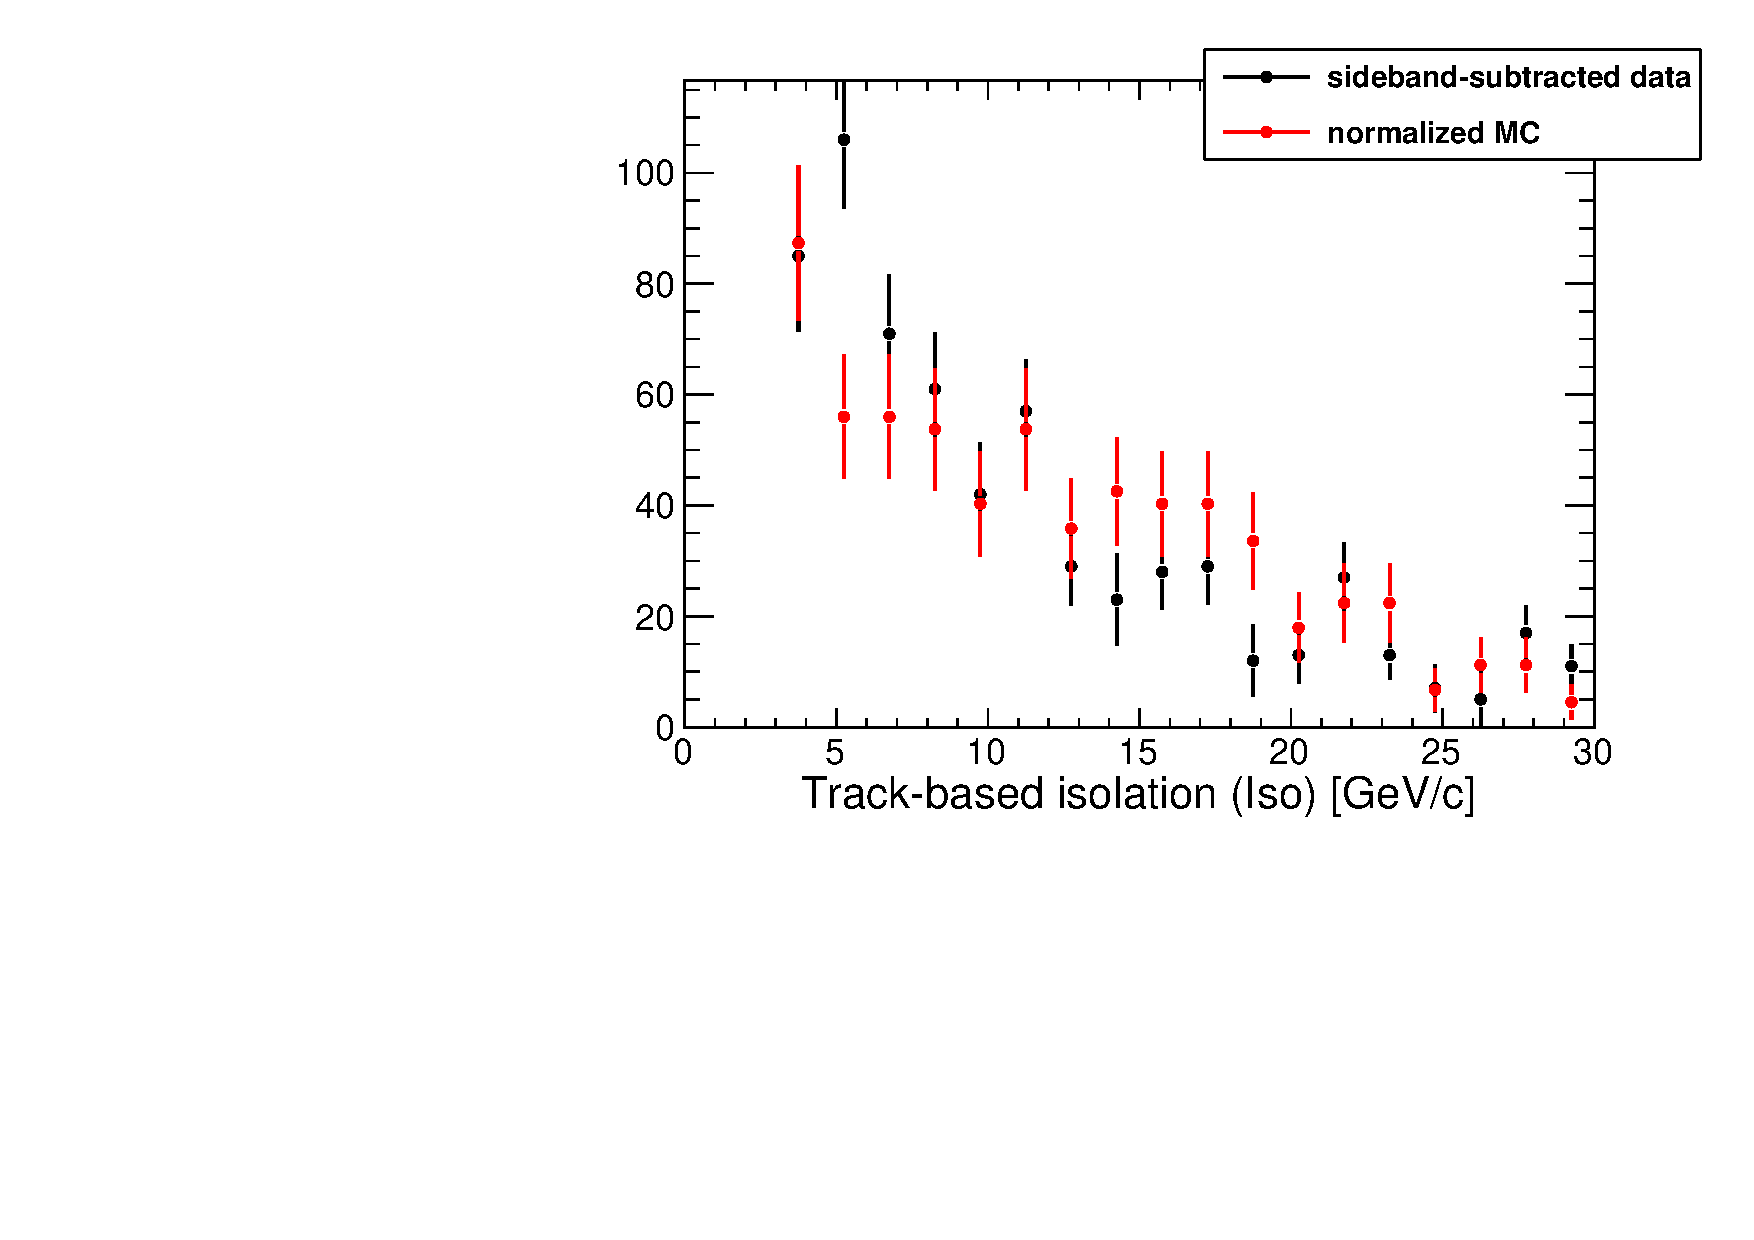
\includegraphics[width=0.45\linewidth]{phi_iso.pdf}
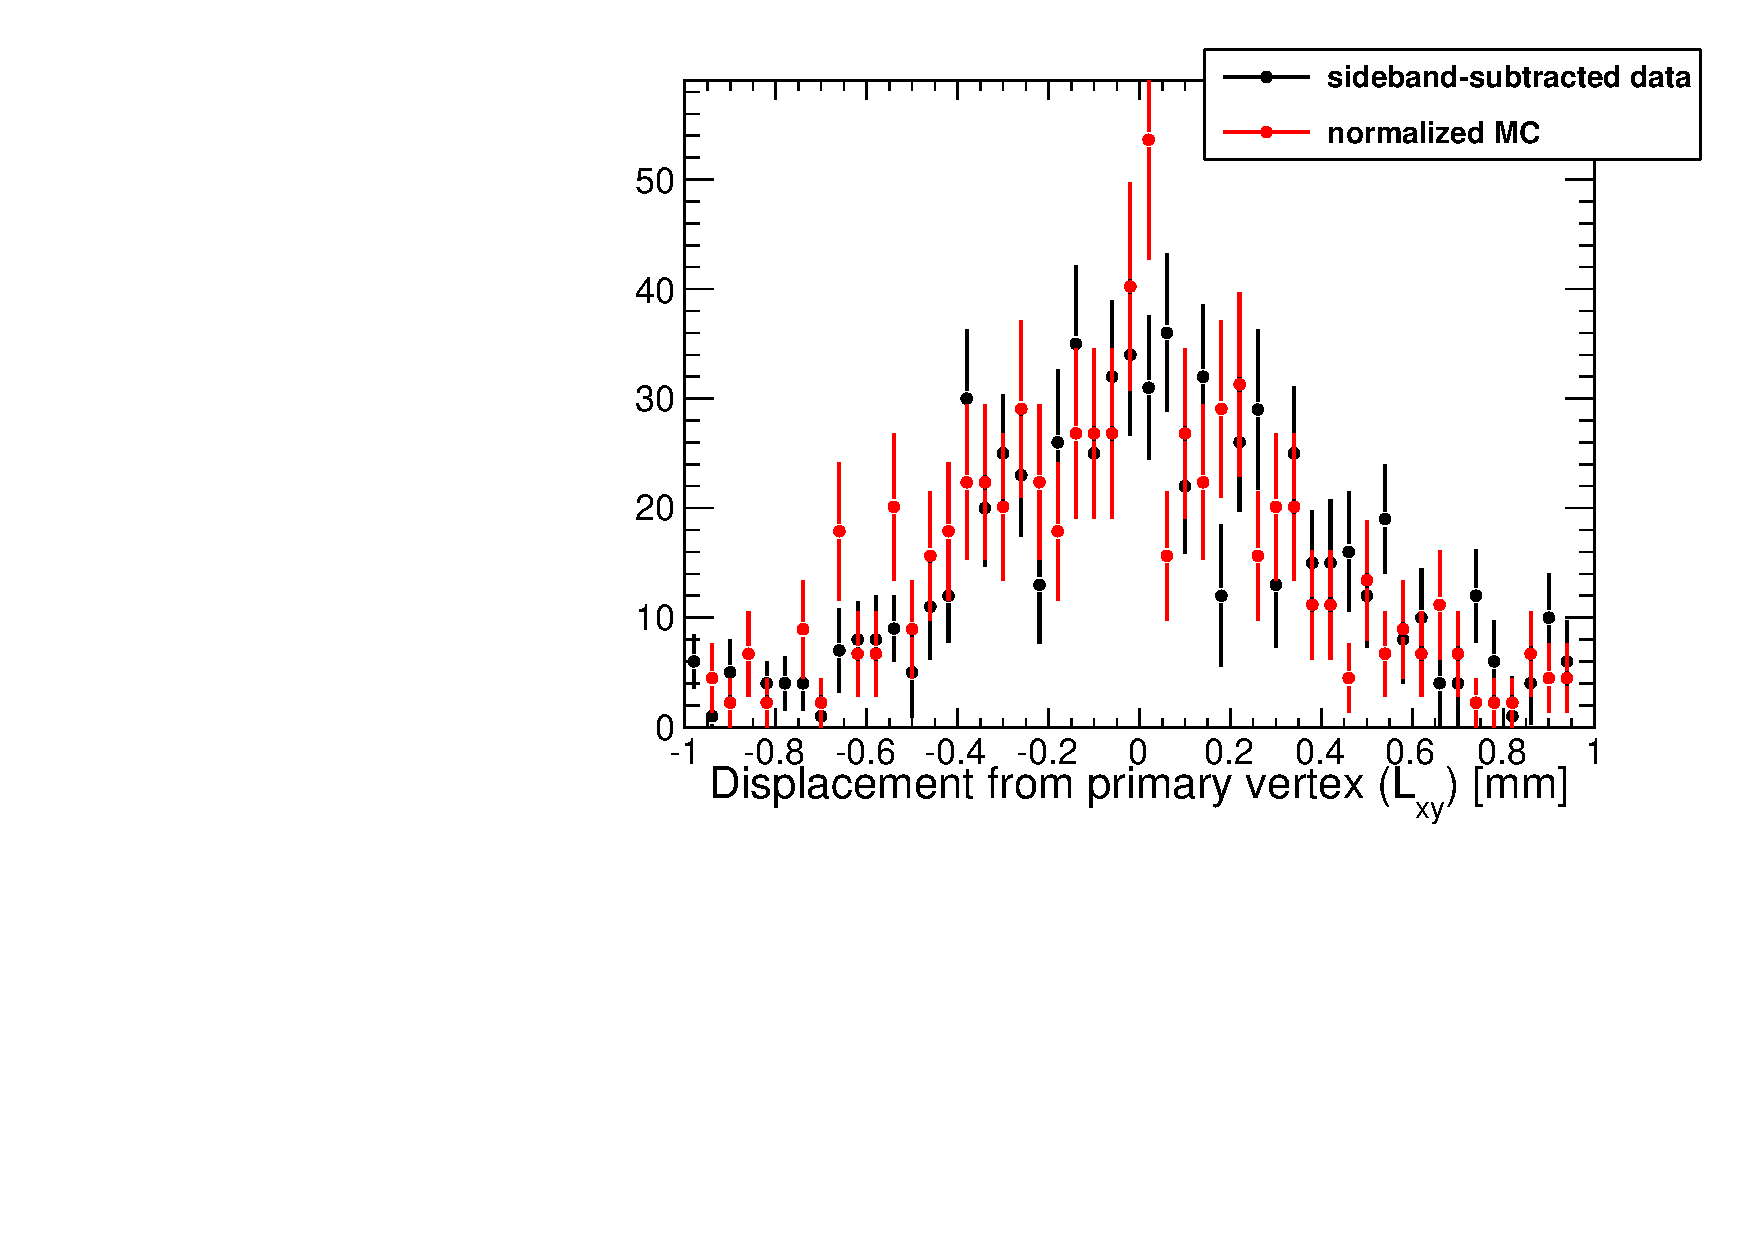
\includegraphics[width=0.45\linewidth]{phi_lxy.pdf}
\end{frame}

%% \section*{First section}
%% \begin{frame}
%% \begin{center}
%% \Huge \textcolor{blue}{First section}
%% \end{center}
%% \end{frame}

\begin{frame}
\frametitle{Conclusions}

\begin{itemize}\setlength{\itemsep}{0.25 cm}
\item In MC, we don't expect significant interference between tracks
  until both muons have $p_T \gtrsim 100$~GeV/$c$ because tracks are
  allowed to share up to 50\% of their hits
\item a $\sim$5\% tracker reconstruction effect is visible for $\Delta R < 0.01$, $p_T > 20$~GeV/$c$
\item interference of nearby muons is a larger effect and applies to a wider range of $\Delta R$ (and is documented in the analysis note)
\item MC simulation reproduces low-level quantities well, and the rest is geometry
\item $\Delta R \sim 0.1$ was tested explicitly using the $\phi(1020)$
  resonance: all in good agreement except normalized $\chi^2$
  distribution, but this difference is well below the cut
\end{itemize}

\label{numpages}
\end{frame}

\end{document}
